\documentclass[12pt]{article}
\usepackage[letterpaper, margin=1in]{geometry}
\usepackage{graphicx}
\graphicspath{{./Figures/}}
\usepackage{hyperref}
\usepackage{parskip}
\usepackage{amsmath}
\usepackage{caption}
\usepackage{subcaption}
\usepackage{enumitem}
\usepackage[framed, numbered]{matlab-prettifier}
\lstset{inputpath=../MATLAB}

\DeclareMathOperator{\sinc}{sinc}
\DeclareMathOperator{\rect}{rect}

\title{ELECENG 3TR4 Lab 4: \\ Random Processes}
\author{
    Aaron Pinto \\ pintoa9
    \and
    Raeed Hassan \\ hassam41
}

% \lstinputlisting[style=Matlab-editor, caption={}, label={}, linerange={}]{Lab4.m} % for reference

\begin{document}

\maketitle
\clearpage

\section*{Numerical Experiment \#1: Evaluation of Autocorrelation and Power Spectral Density}

\begin{enumerate}[label=\roman*)]
	\item % (i) calculate the theoretical autocorrelation function of the output, and the corresponding PSD using the methodology discussed in class. Compare (qualitatively) your theoretical results with those from your program, and explain any discrepancies. Note that the amplitude (i.e. y-axis) of PSD of the matlab could be different from that of the theoretical PSD because of the difference between DFT and Fourier transform.
	The theoretical autocorrelation function of the output is derived in Equation~\ref{eq:exp1_autocorr}.
	\begin{equation} \label{eq:exp1_autocorr}
	\begin{aligned}[b]
			y(n) &= h(n)\ast w(n) \\
			h(n) &= 2B\sinc(2Bn) \\
			&= 2\cdot 250sinc(2\cdot 250 n) \\
			R_y(m) &= E\left[y(n)\cdot y(n+m)\right] \\
			&= \sum_k\sum_j h(k)h(j)E[w(n-k)w(n+m-j)] \\
			&= \sum_k h(k)h(k+m)\sigma_w^2 \\
			&= \sum_k (500\sinc(500k))(500\sinc(500(k+m)))\sigma_w^2 \\
			&= \sum_k 250000\sinc(500k)\sinc(500(k+m))\sigma_w^2 \\
	\end{aligned}
	\end{equation}
	The PSD is just the Fourier transform of the autocorrelation function. The PSD is derived in Equation~\ref{eq:exp1_psd}, where k is the gain of the noise.
	\begin{equation} \label{eq:exp1_psd}
	\begin{aligned}[b]
			S_y(f) &= k \left | H(f) \right |^2 \\
			&= k \rect(\frac{f}{2\cdot 250}) \\
			&= k \rect(\frac{f}{500}) \\
	\end{aligned}
	\end{equation}

	The theoretical results from Equation~\ref{eq:exp1_autocorr} and Equation~\ref{eq:exp1_psd} can be compared to the results of the numerical experiment in Figure~\ref{fig:exp1_maxlag100}. We can see that both the autocorrelation and PSD match between the theoretical results and the numerical results. Both autocorrelation functions result in $\sinc$ functions with the same frequency. Similarly, both PSDs produce a $\rect$ function with a bandwidth of 250 Hz, although is noise in the passband of the MATLAB PSD, as the signal used for the MATLAB plot does not use an ideal white noise signal.

	\item % (ii) change the maxlag from 100 to 200 and then to 500 and observe its impact on the PSD and comment. Include plots of all relevant quantities.
	We can see the impact of increasing the maxlag to 200 in Figure~\ref{fig:exp1_maxlag200} and increasing the maxlag to 500 in Figure~\ref{fig:exp1_maxlag500}. We can see that there is more information in the PSD as we increase the maxlag, as doing so increases the frequency resolution of our PSD.

	\item % (iii) Estimate the bandwidth of the filter using the autocorrelation plot. Hint: measure the locations of zeros of sinc and compare it with the theoretical calculation. 
	We can estimate the bandwidth of the filter using the autocorrelation plot. We can see that in all three plots of the autocorrelation function, the zeros of the $\sinc$ function are spaced $0.002$ seconds apart. This means the $\sinc$ function repeats peaks and troughs every $0.004$ seconds. We can determine the bandwidth of the filter to be $\frac{1}{0.004\text{ s}}$ or 250 Hz.

	\begin{figure}[h]
		\centering
		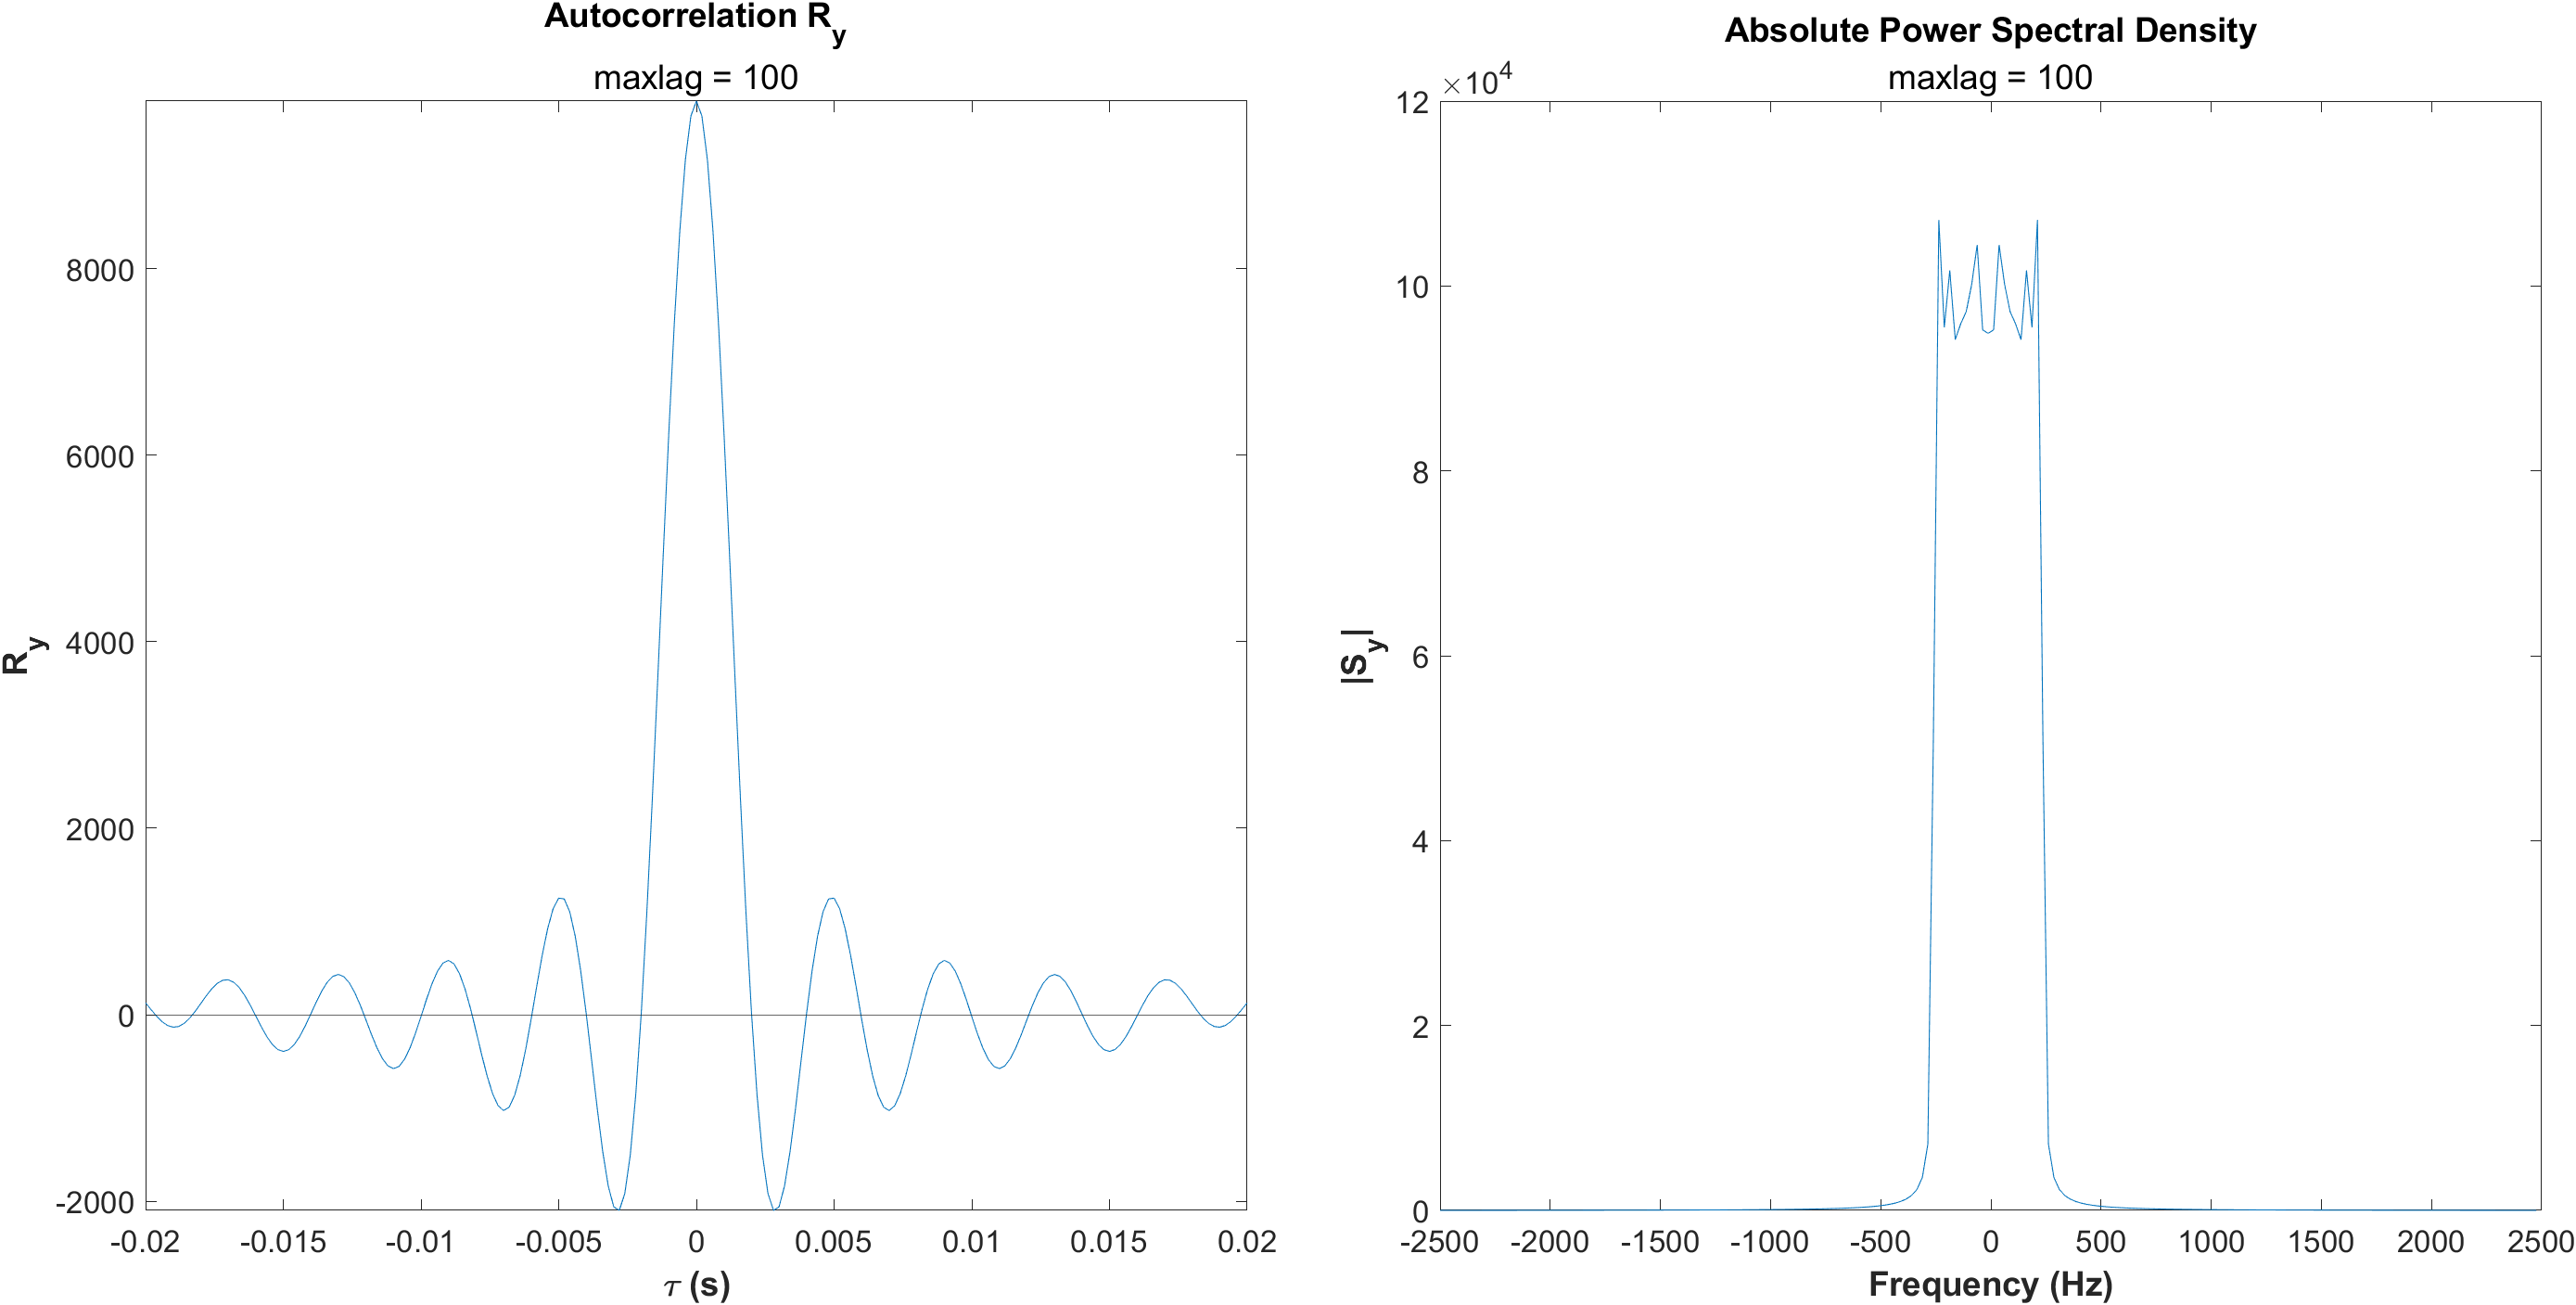
\includegraphics[width=0.78\textwidth]{exp1_maxlag_100}
		\caption{\label{fig:exp1_maxlag100}Autocorrelation and PSD for maxlag = 100}
	\end{figure}

	\begin{figure}[h]
		\centering
		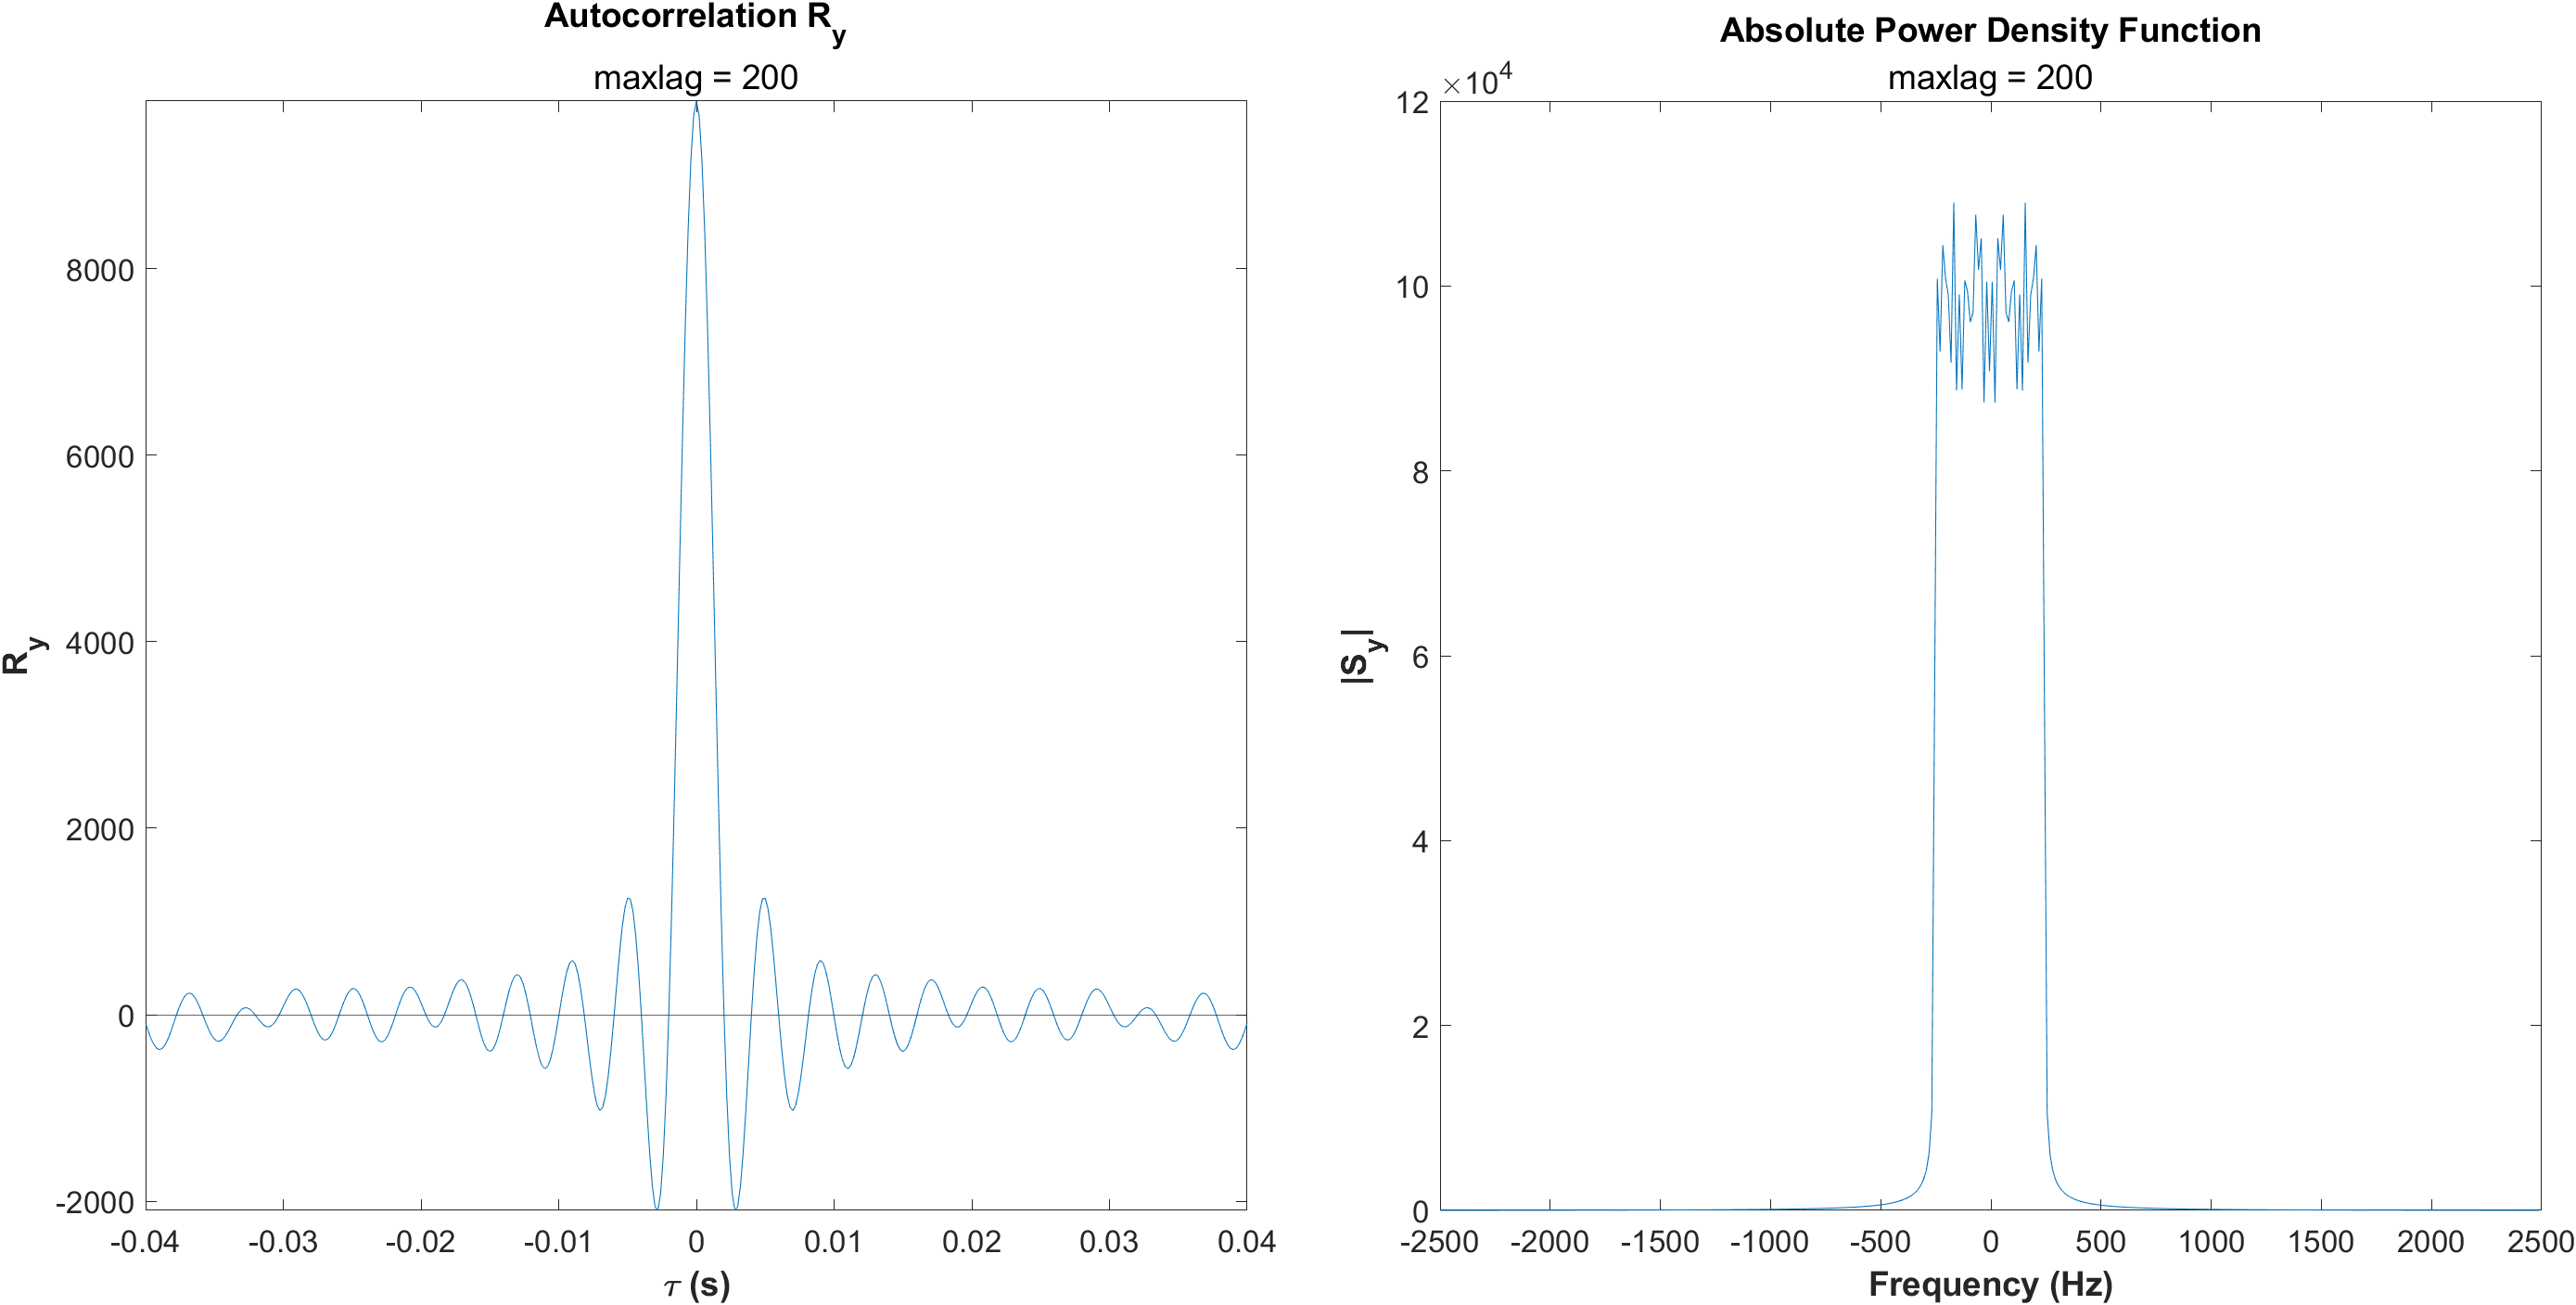
\includegraphics[width=0.78\textwidth]{exp1_maxlag_200}
		\caption{\label{fig:exp1_maxlag200}Autocorrelation and PSD for maxlag = 200}
	\end{figure}
	
	\begin{figure}[h]
		\centering
		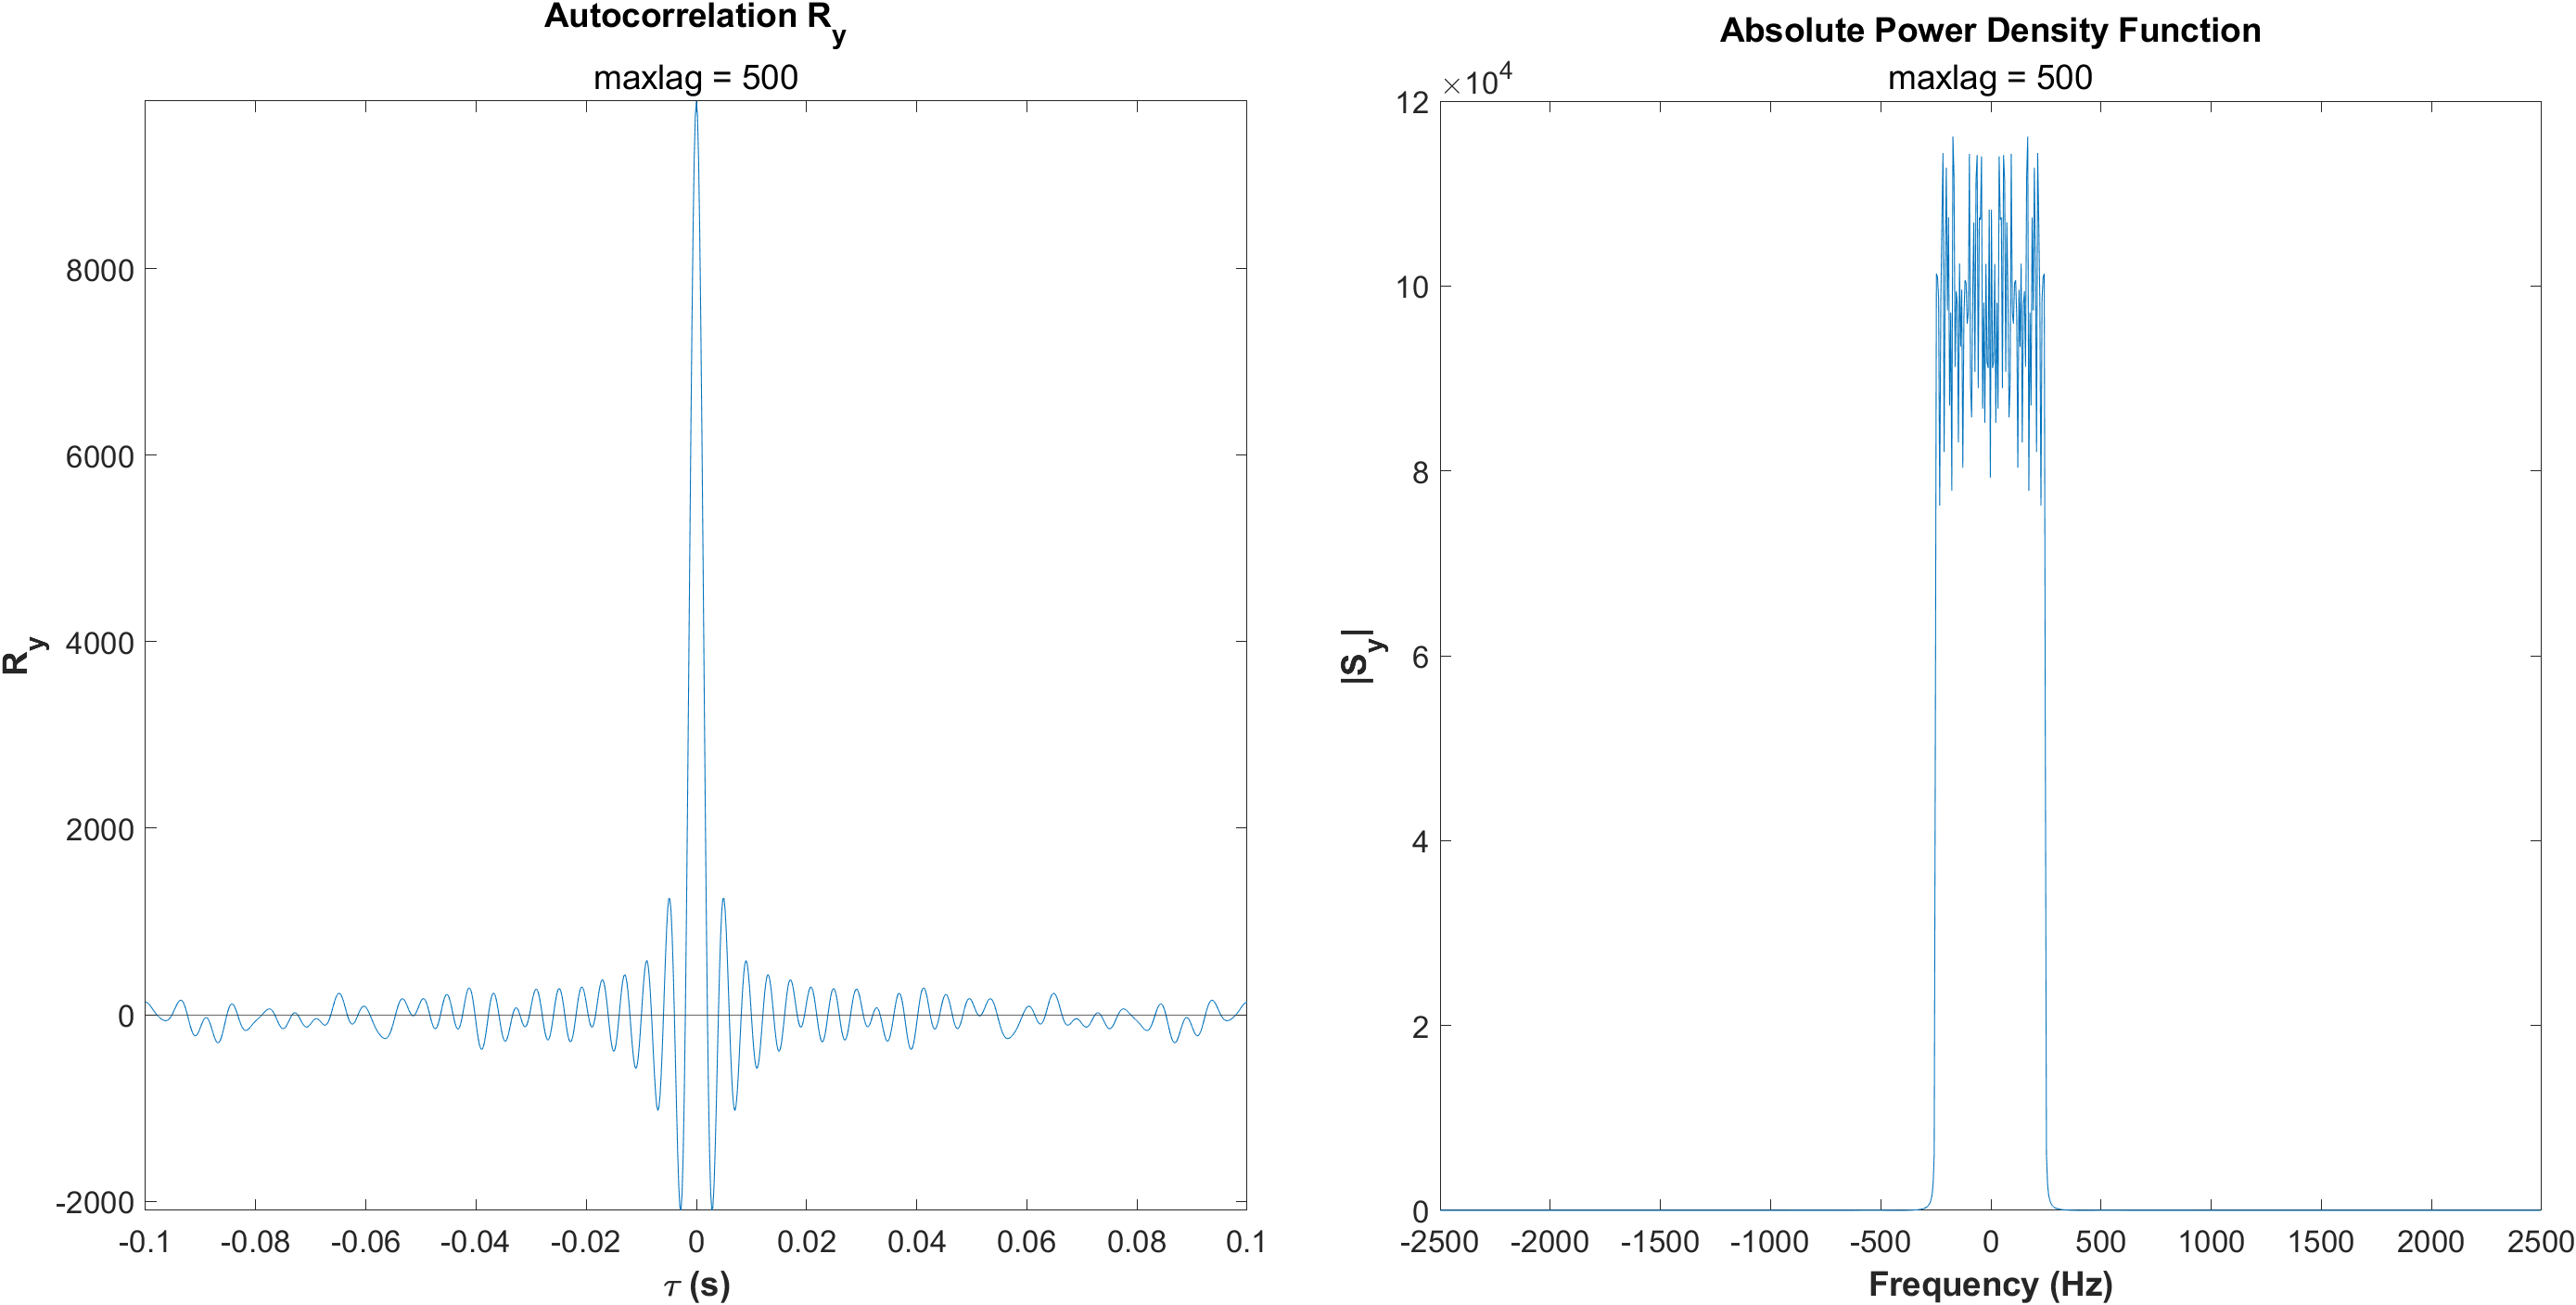
\includegraphics[width=0.78\textwidth]{exp1_maxlag_500}
		\caption{\label{fig:exp1_maxlag500}Autocorrelation and PSD for maxlag = 500}
	\end{figure}

\end{enumerate} \clearpage

\section*{Numerical Experiment \#2: A sinusoid buried in noise}

% For this section, provide the theoretical calculations (i.e. derivations of analytical expressions for autocorrelation and PSD of the AWGN channel output. Refer to lecture notes). Compare the theoretical autocorrelation function and PSD with those from your program (qualitatively).

The theoretical autocorrelation function of the output is derived in Equation~\ref{eq:exp2_autocorr}.
\begin{equation} \label{eq:exp2_autocorr}
\begin{aligned}[b]
	y(t) &= A\sin(2\pi f_ct + \theta) + w(t) \\
	R_y(\tau) &= E\left\{y(t)y(t+\tau)\right\} \\
	&= E\left \{\left[ A\sin(\underbrace{2 \pi f_c t + \theta}_{x}) + w(t) \right]\cdot \left[ A\sin(\underbrace{2 \pi f_c (t+\tau) + \theta}_{y}) + w(t+\tau) \right] \right \} \\
	&= E\left \{A^2\sin(x)\sin(y) + A\sin(x)\cdot w(t+\tau) + w(t)\cdot A\sin(y) + w(t)\cdot w(t+\tau)\right \} \\
	&= \frac{A^2}{2}\sin(2\pi f_c \tau) + 0 + 0 + \frac{N_0}{2}\delta(\tau) \\
	&= \frac{A^2}{2} \sin(2\pi f_c \tau) + \frac{N_0}{2}\delta(\tau) \\
\end{aligned}
\end{equation}

The PSD is just the Fourier transform of the autocorrelation function. The PSD is derived in Equation~\ref{eq:exp2_psd}.
\begin{equation} \label{eq:exp2_psd}
\begin{aligned}[b]
	R_y(\tau) &= \frac{A^2}{2} \sin(2\pi f_c \tau) + \frac{N_0}{2}\delta(\tau) \\
	S_y(f) &= \left |F\left \{\frac{A^2}{2} \sin(2\pi f_c \tau) \right \} + F\left \{\frac{N_0}{2}\delta(\tau) \right \}\right | \\
	&= \left | i \cdot \frac{A^2}{4} \left [\delta(f - f_c) - \delta(f + f_c)\right ]\right | + \frac{N_0}{2} \\
	&= \frac{A^2}{4} \left [\delta(f - f_c) - \delta(f + f_c)\right ] + \frac{N_0}{2}
\end{aligned}
\end{equation}

The theoretical results from Equation~\ref{eq:exp2_autocorr} and Equation~\ref{eq:exp2_psd} can be compared to the results of the numerical experiment in Figure~\ref{fig:exp2_maxlag100}. We can see that both the autocorrelation and PSD match between the theoretical results and the numerical results. Both autocorrelation functions result in $\sin$ functions with an impulse at $\tau = 0$. Similarly, both PSDs produce two impulses at what should be $-f_c$ and $f_c$, with a floor caused by the noise.

\begin{enumerate}[label=\roman*)]
	\item % (i) Do you observe a peak at the zero lag in the autocorrelation plot? Explain its origin.
	There is a peak at the zero lag in the autocorrelation plot. This peak is caused by the impulse in the autocorrelation function due to the white noise.

	\item % (ii) Change the maxlag from 100 to 200 and then to 20000and observe its impact on the frequency resolution. Estimating the frequency, fc in the frequency domain and provide a table of measurements for the maxlag of 100, 200 and 20000. Do the frequency estimates converge? Explain the connection between the maxlog and frequency resolution.

	We can see the impact of increasing the maxlag to 200 in Figure~\ref{fig:exp2_maxlag200} and increasing the maxlag to 20000 in Figure~\ref{fig:exp2_maxlag2000}. As we increase the maxlag the frequency resolution of the PSD increases, resulting in narrower peaks in the PSD plots. A table of measurements for the measured frequency estimates for $f_c$ at each maxlag value is shown in Table~\ref{table:exp2}. We can see that as the value of maxlag increases, the frequency estimate for $f_c$ approaches 250 Hz due the the increase in frequency resolution. As maxlag increases, the size of the $\tau$ vector increases. The size of the frequency vector is dependent on the size of the $\tau$ vector. As the range of the frequency vector does not change, the increase in the number of frequency samples in the vector due to an increase maxlag increases the resolution of the frequency vector.

	\begin{table}[h]
		\centering
		\begin{tabular}{c|c}
			maxlag & $f_c$  \\ \hline
			100    & 236.32 \\
			200    & 243.14 \\
			20000  & 249.93
		\end{tabular}
		\caption{\label{table:exp2}Table of Measurements of maxlag and $f_c$}
	\end{table}

	\begin{figure}[h]
		\centering
		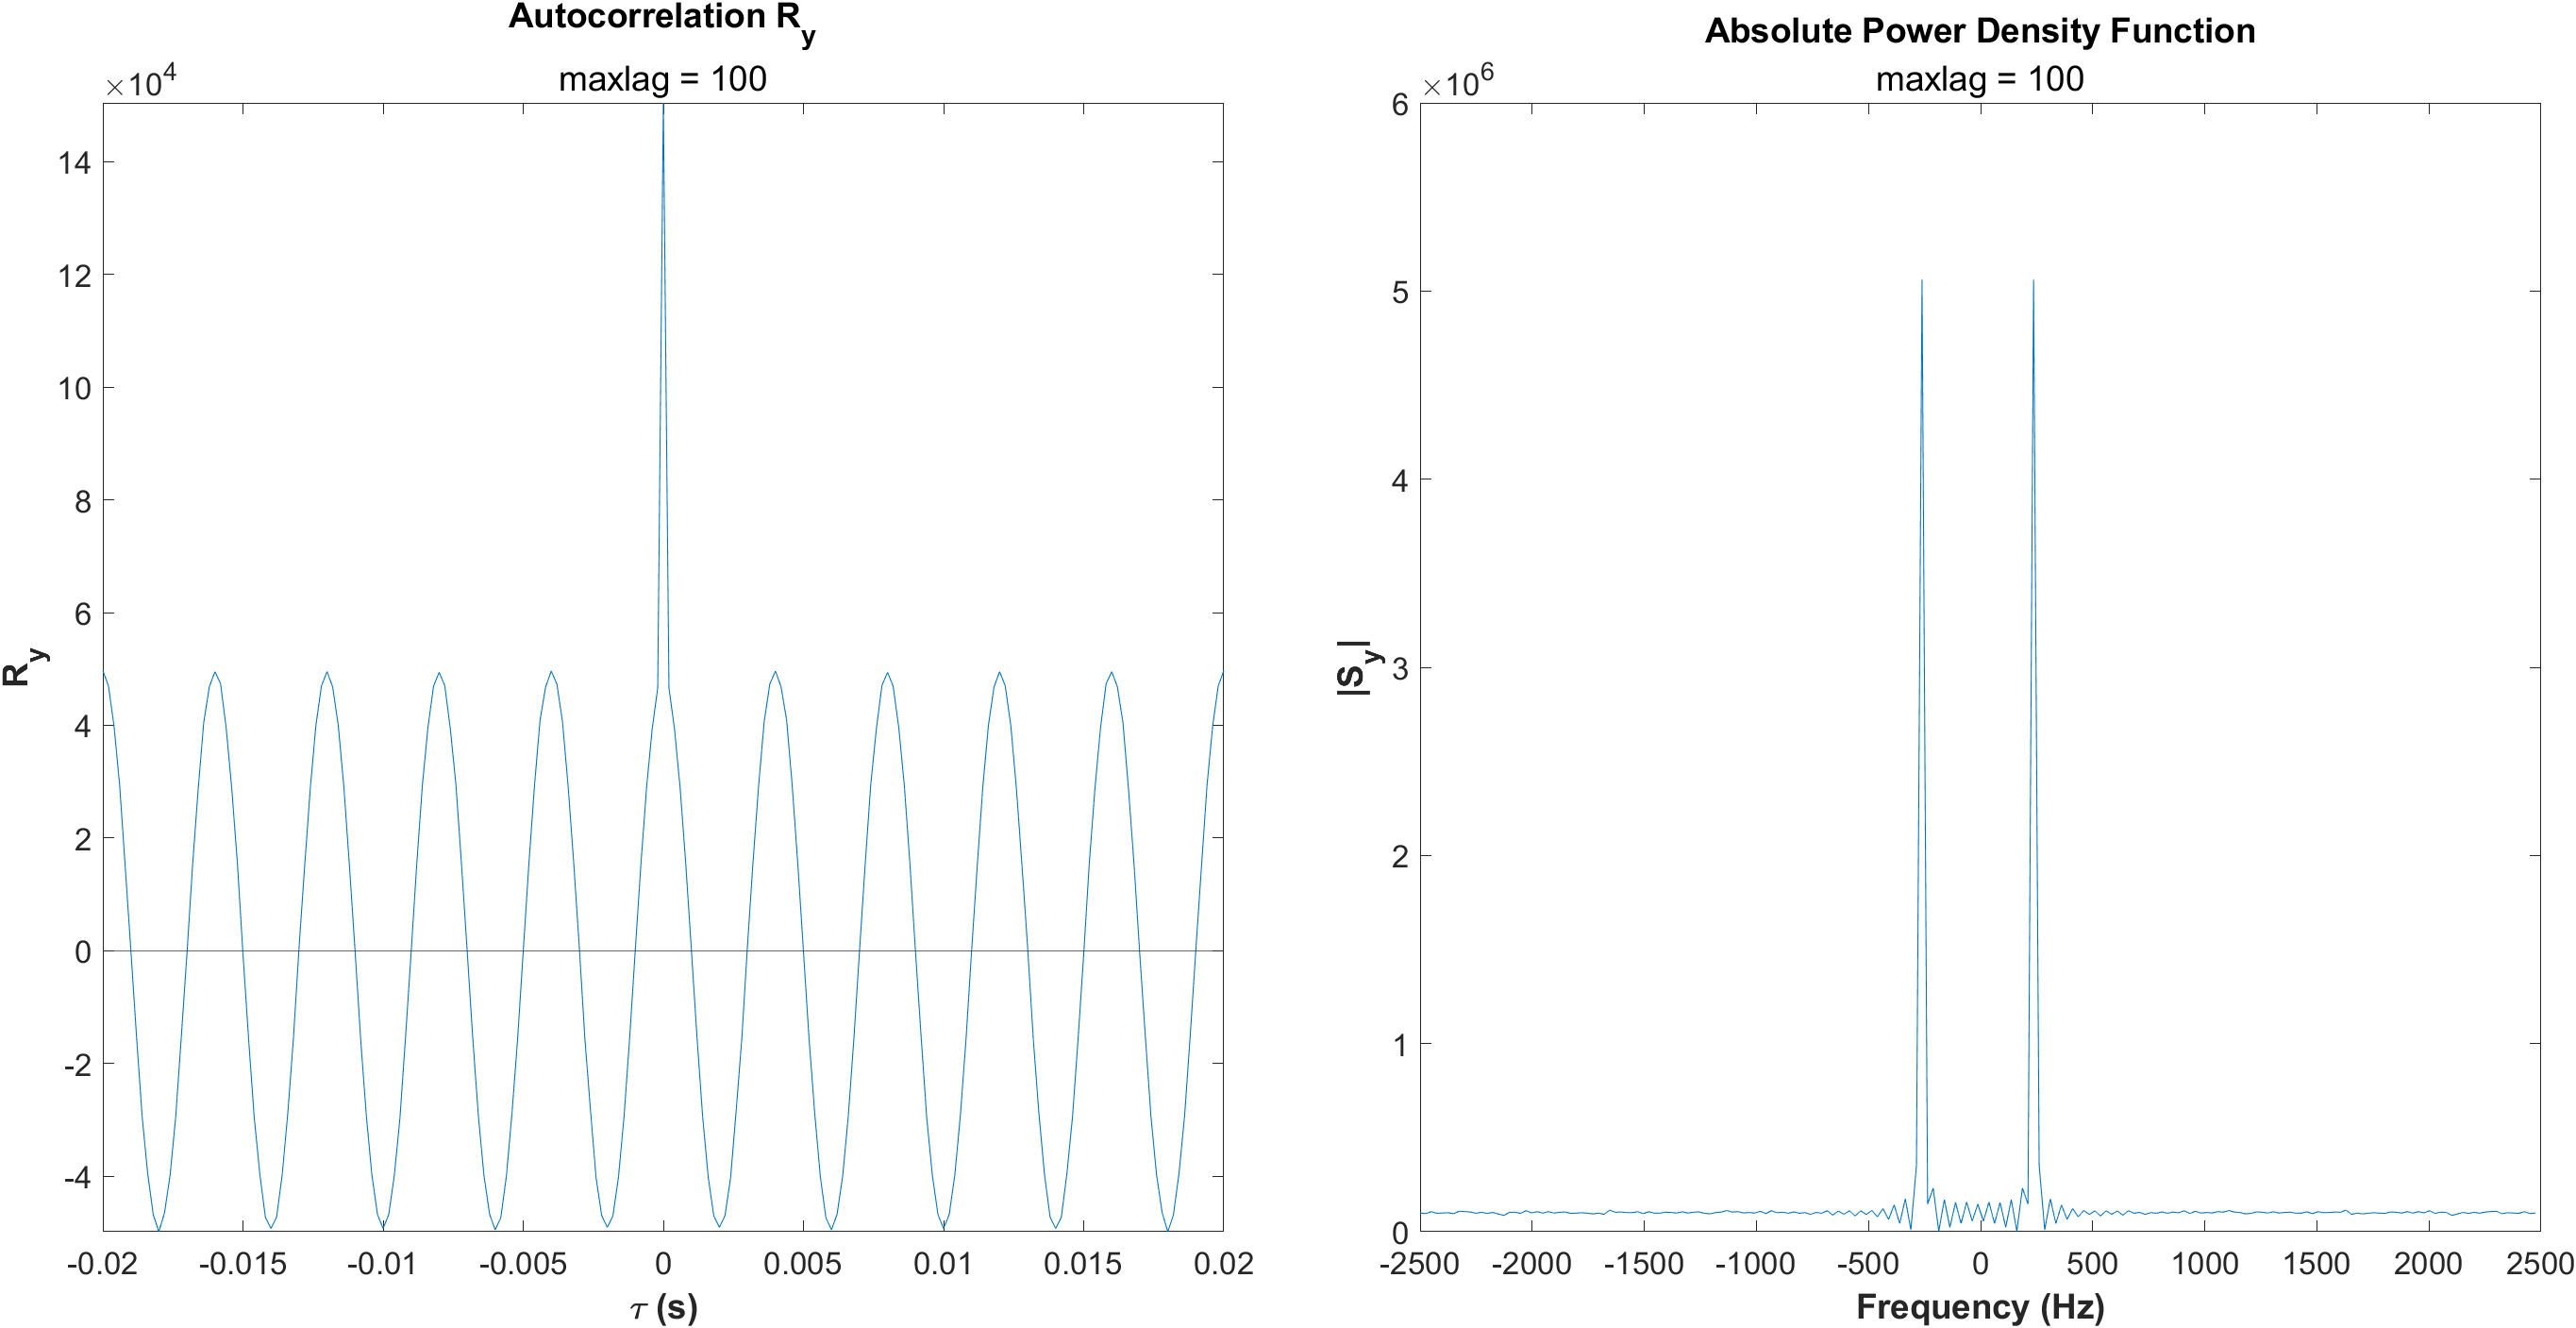
\includegraphics[width=\textwidth]{exp2_maxlag_100}
		\caption{\label{fig:exp2_maxlag100}Autocorrelation and PSD for maxlag = 100}
	\end{figure}

	\begin{figure}[h]
		\centering
		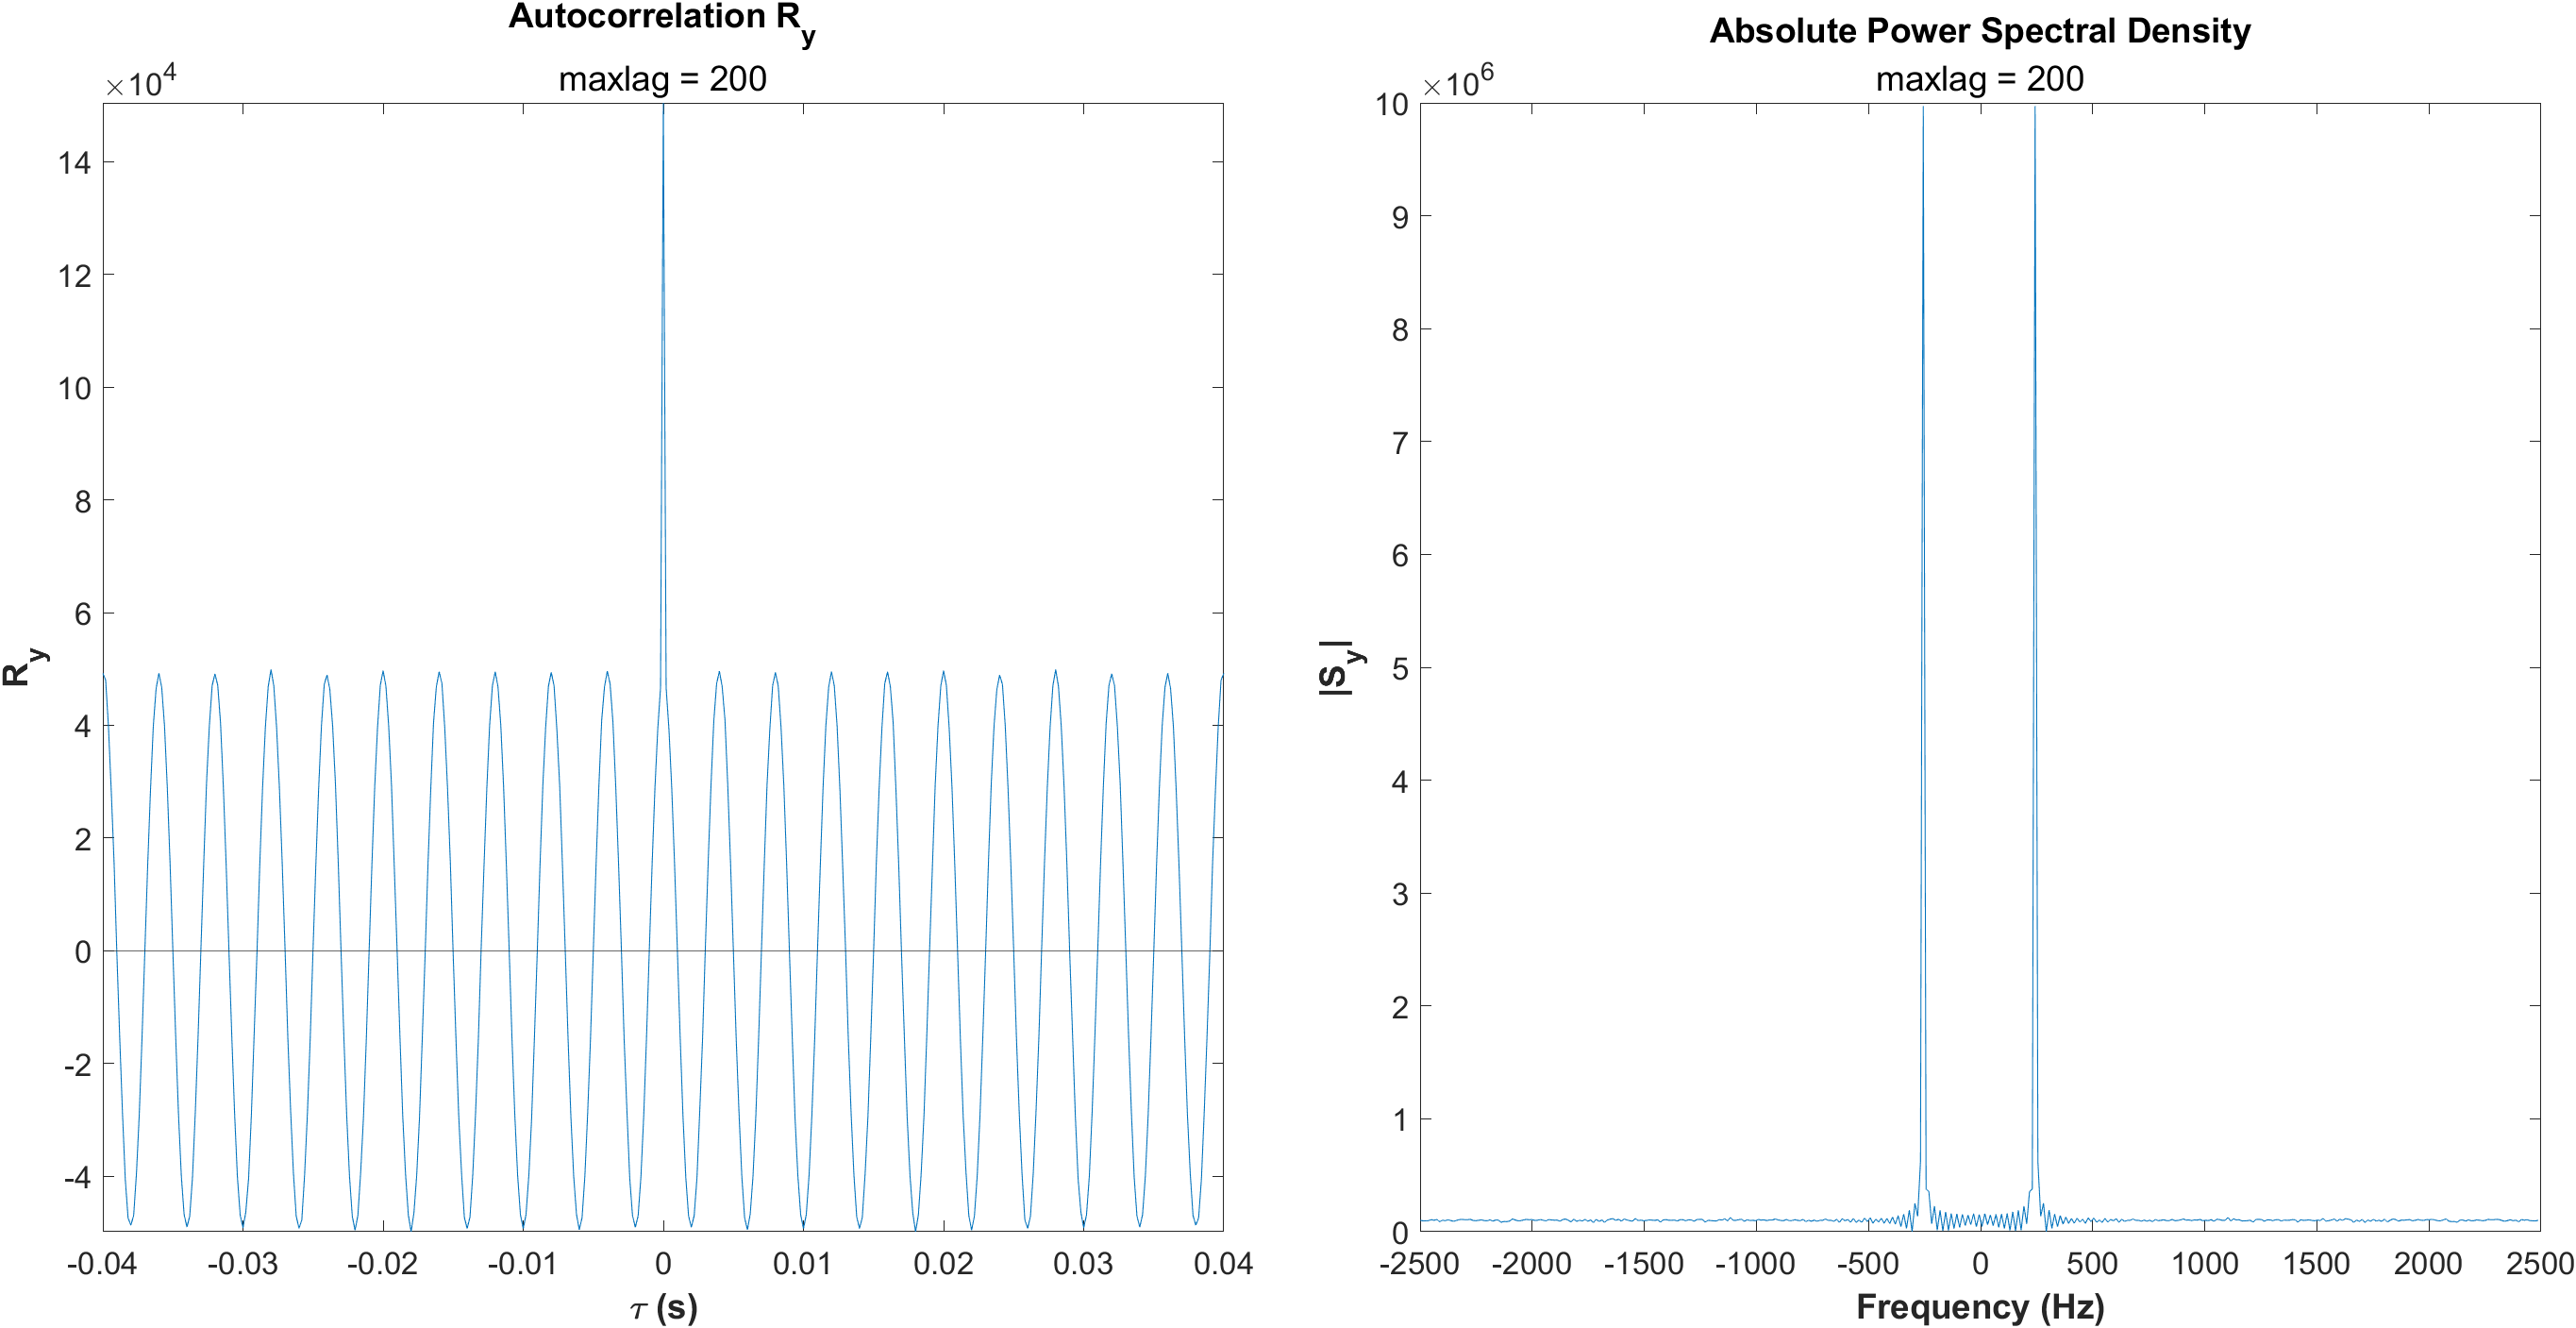
\includegraphics[width=\textwidth]{exp2_maxlag_200}
		\caption{\label{fig:exp2_maxlag200}Autocorrelation and PSD for maxlag = 200}
	\end{figure}

	\clearpage
	
	\begin{figure}[h]
		\centering
		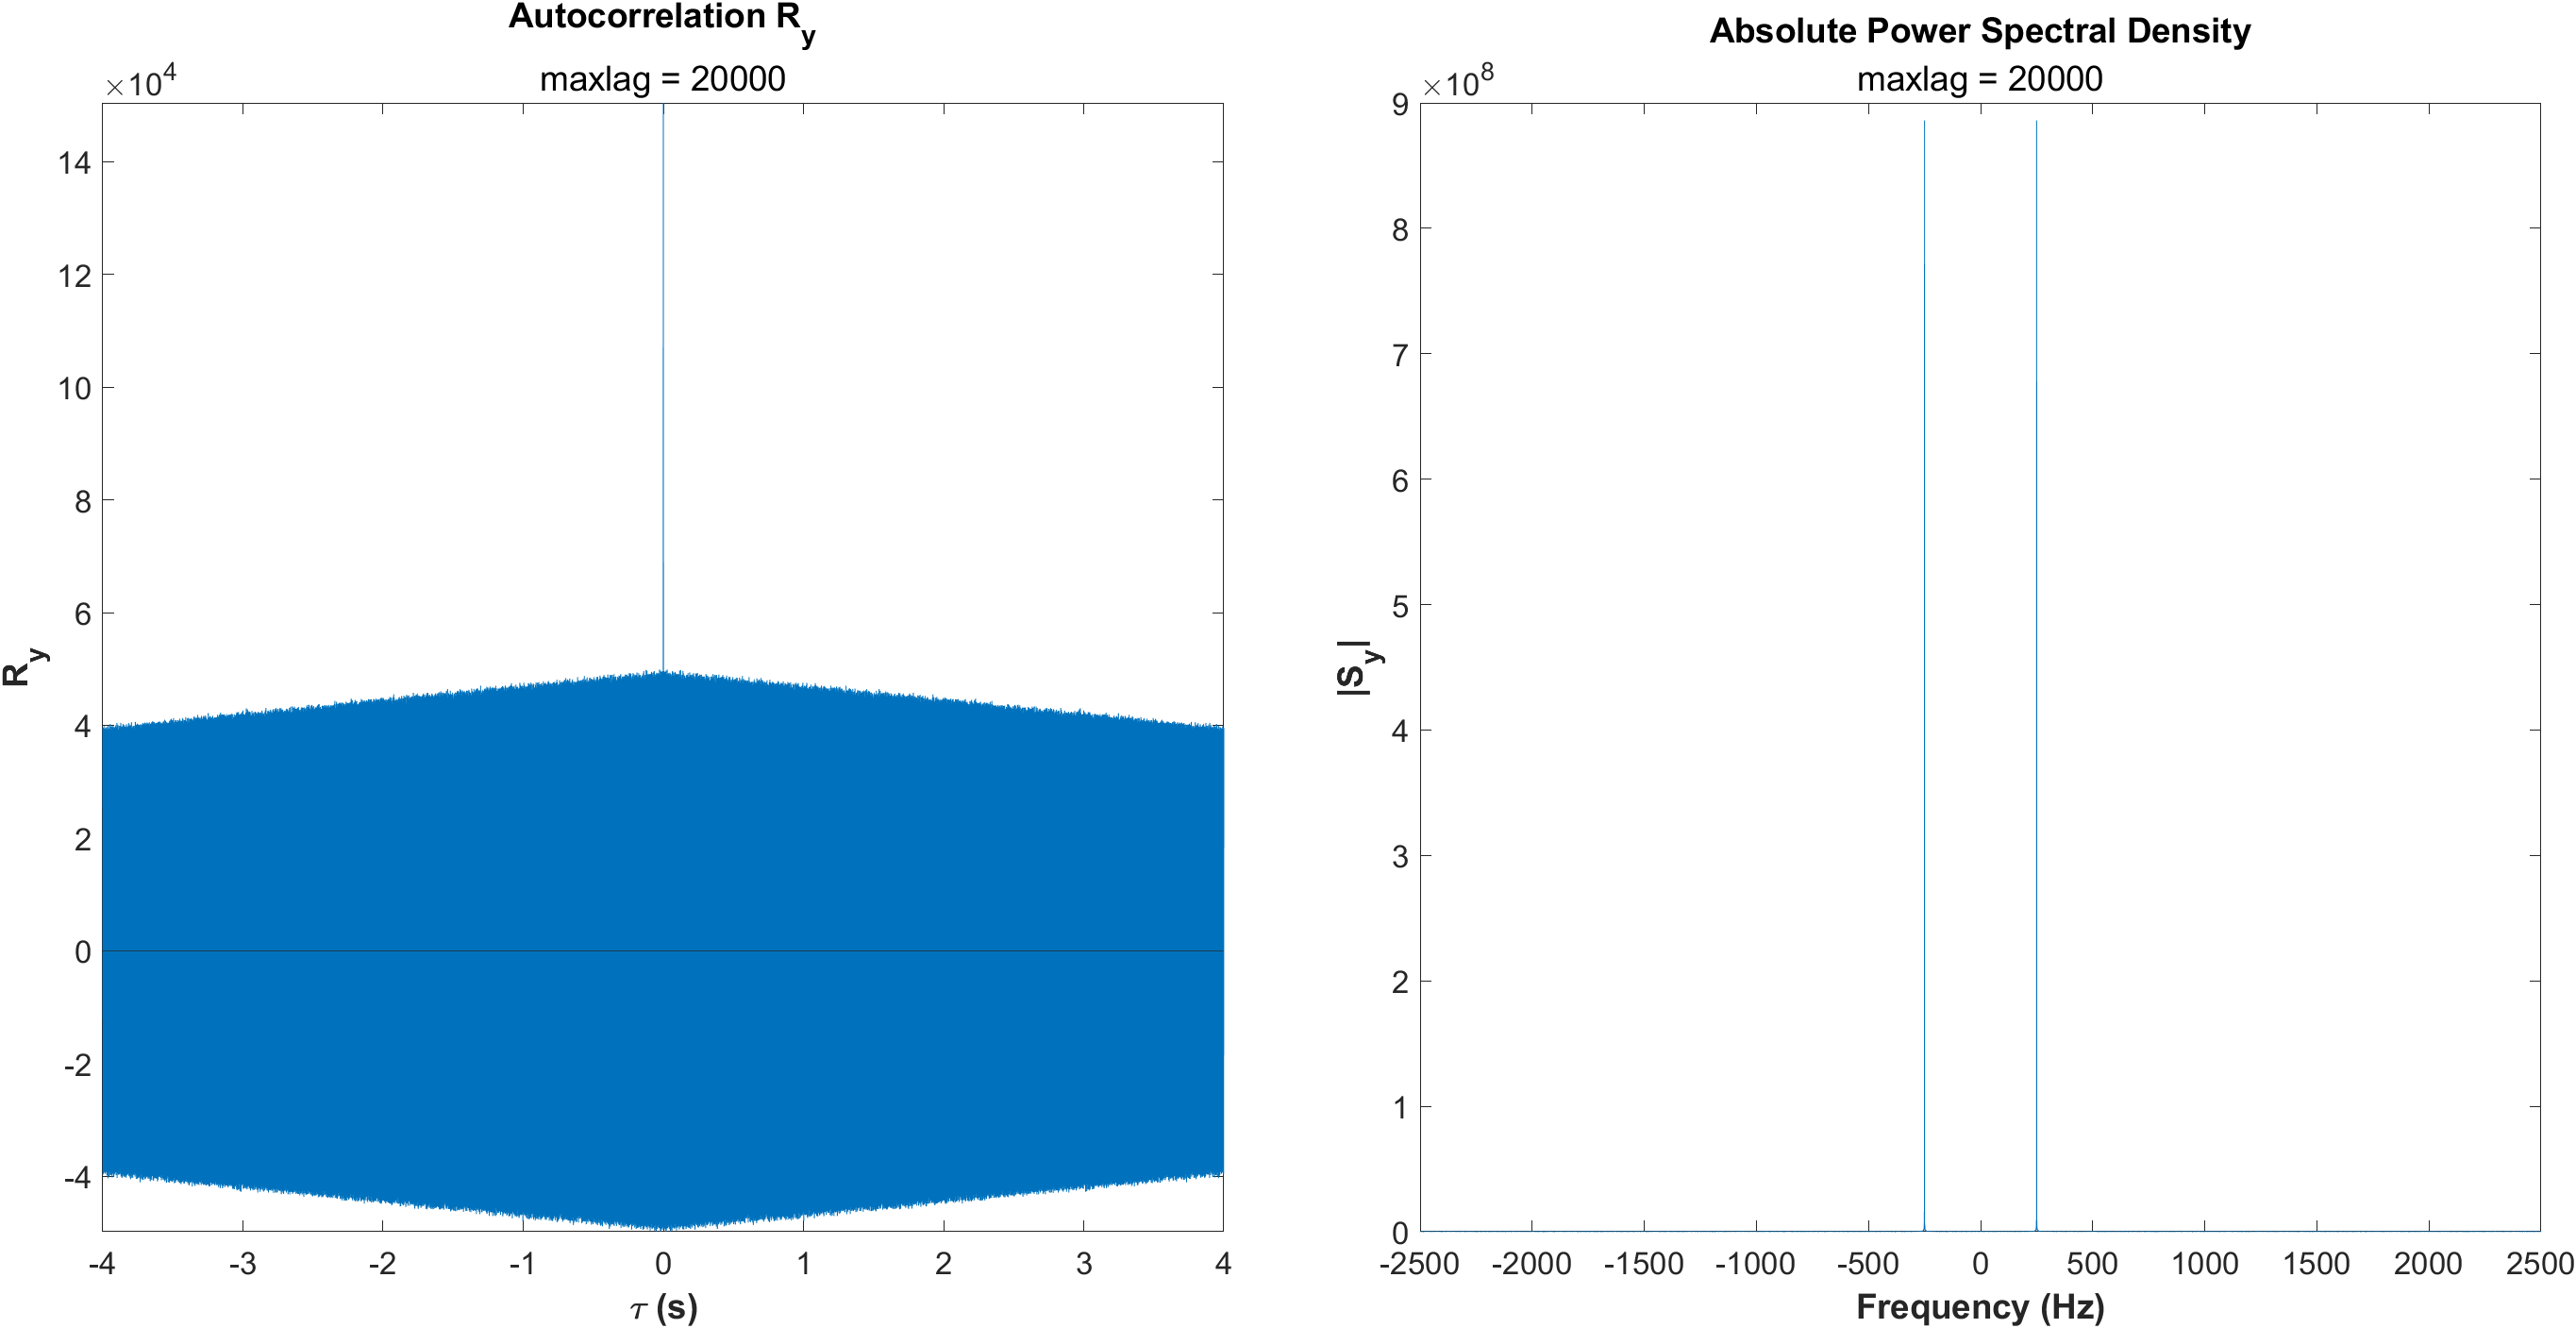
\includegraphics[width=0.8\textwidth]{exp2_maxlag_20000}
		\caption{\label{fig:exp2_maxlag2000}Autocorrelation and PSD for maxlag = 20000}
	\end{figure}

	\item % (iii) Plot yt as a function of time. It is the sinusoidal signal buried in noise (i.e. x(t) plus white noise). Can you estimate the frequency, fc directly from yt, without calculating the correlation? Explain.
	The signal $yt$ is plotted as a function of time in Figure~\ref{fig:exp2_time}. We can see that the sinusoidal signal is buried in noise. We can estimate the frequency $f_c$ directly from $yt$ by taking the FFT of $yt$. We can clearly see in the FFT of $yt$ shown in Figure~\ref{fig:exp2_fft} that the frequency $f_c$ of the output signal $yt$ is around 250 Hz, which matches our $f_c$ estimates from after calculating the correlation. However, if the signal was buried in even more noise, it might not be possible to recover the signal with this methodology. In this case, it could even be possible to estimate the frequency of the signal by looking at the output signal $yt$ in the time domain in Figure~\ref{fig:exp2_time}.

	\begin{figure}[h]
		\centering
		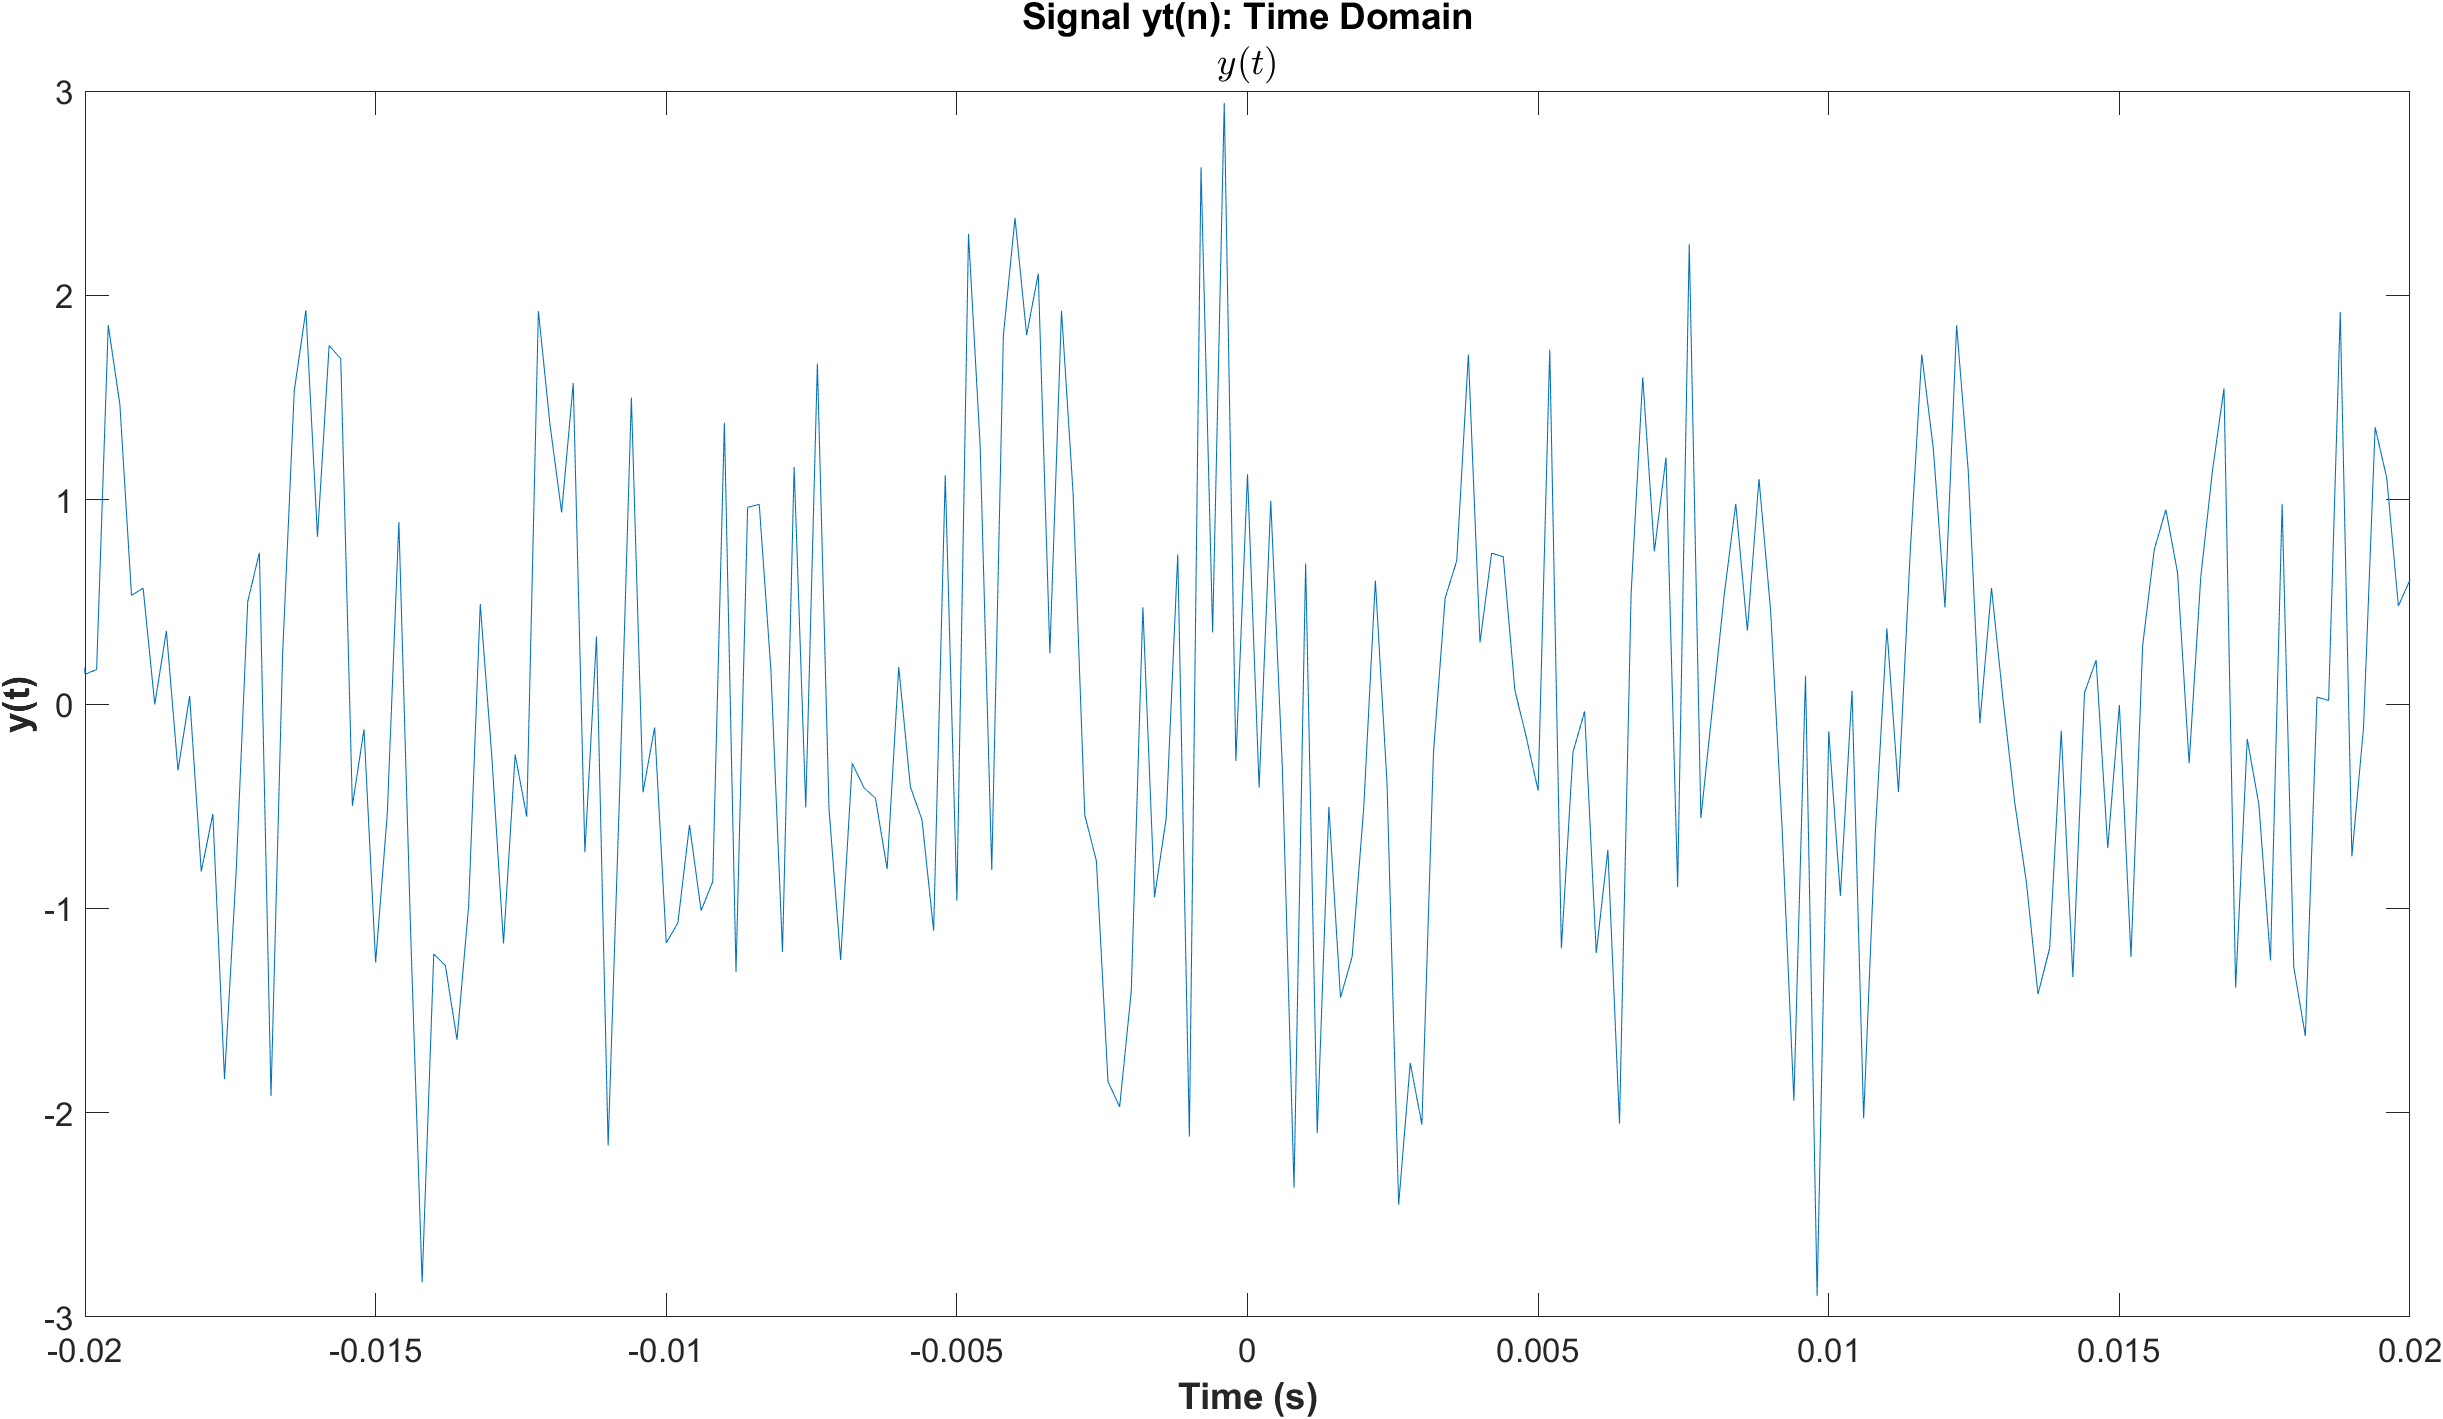
\includegraphics[width=0.86\textwidth]{exp2_time}
		\caption{\label{fig:exp2_time}Signal $yt$: Time Domain}
	\end{figure}

	\clearpage

	\begin{figure}[h]
		\centering
		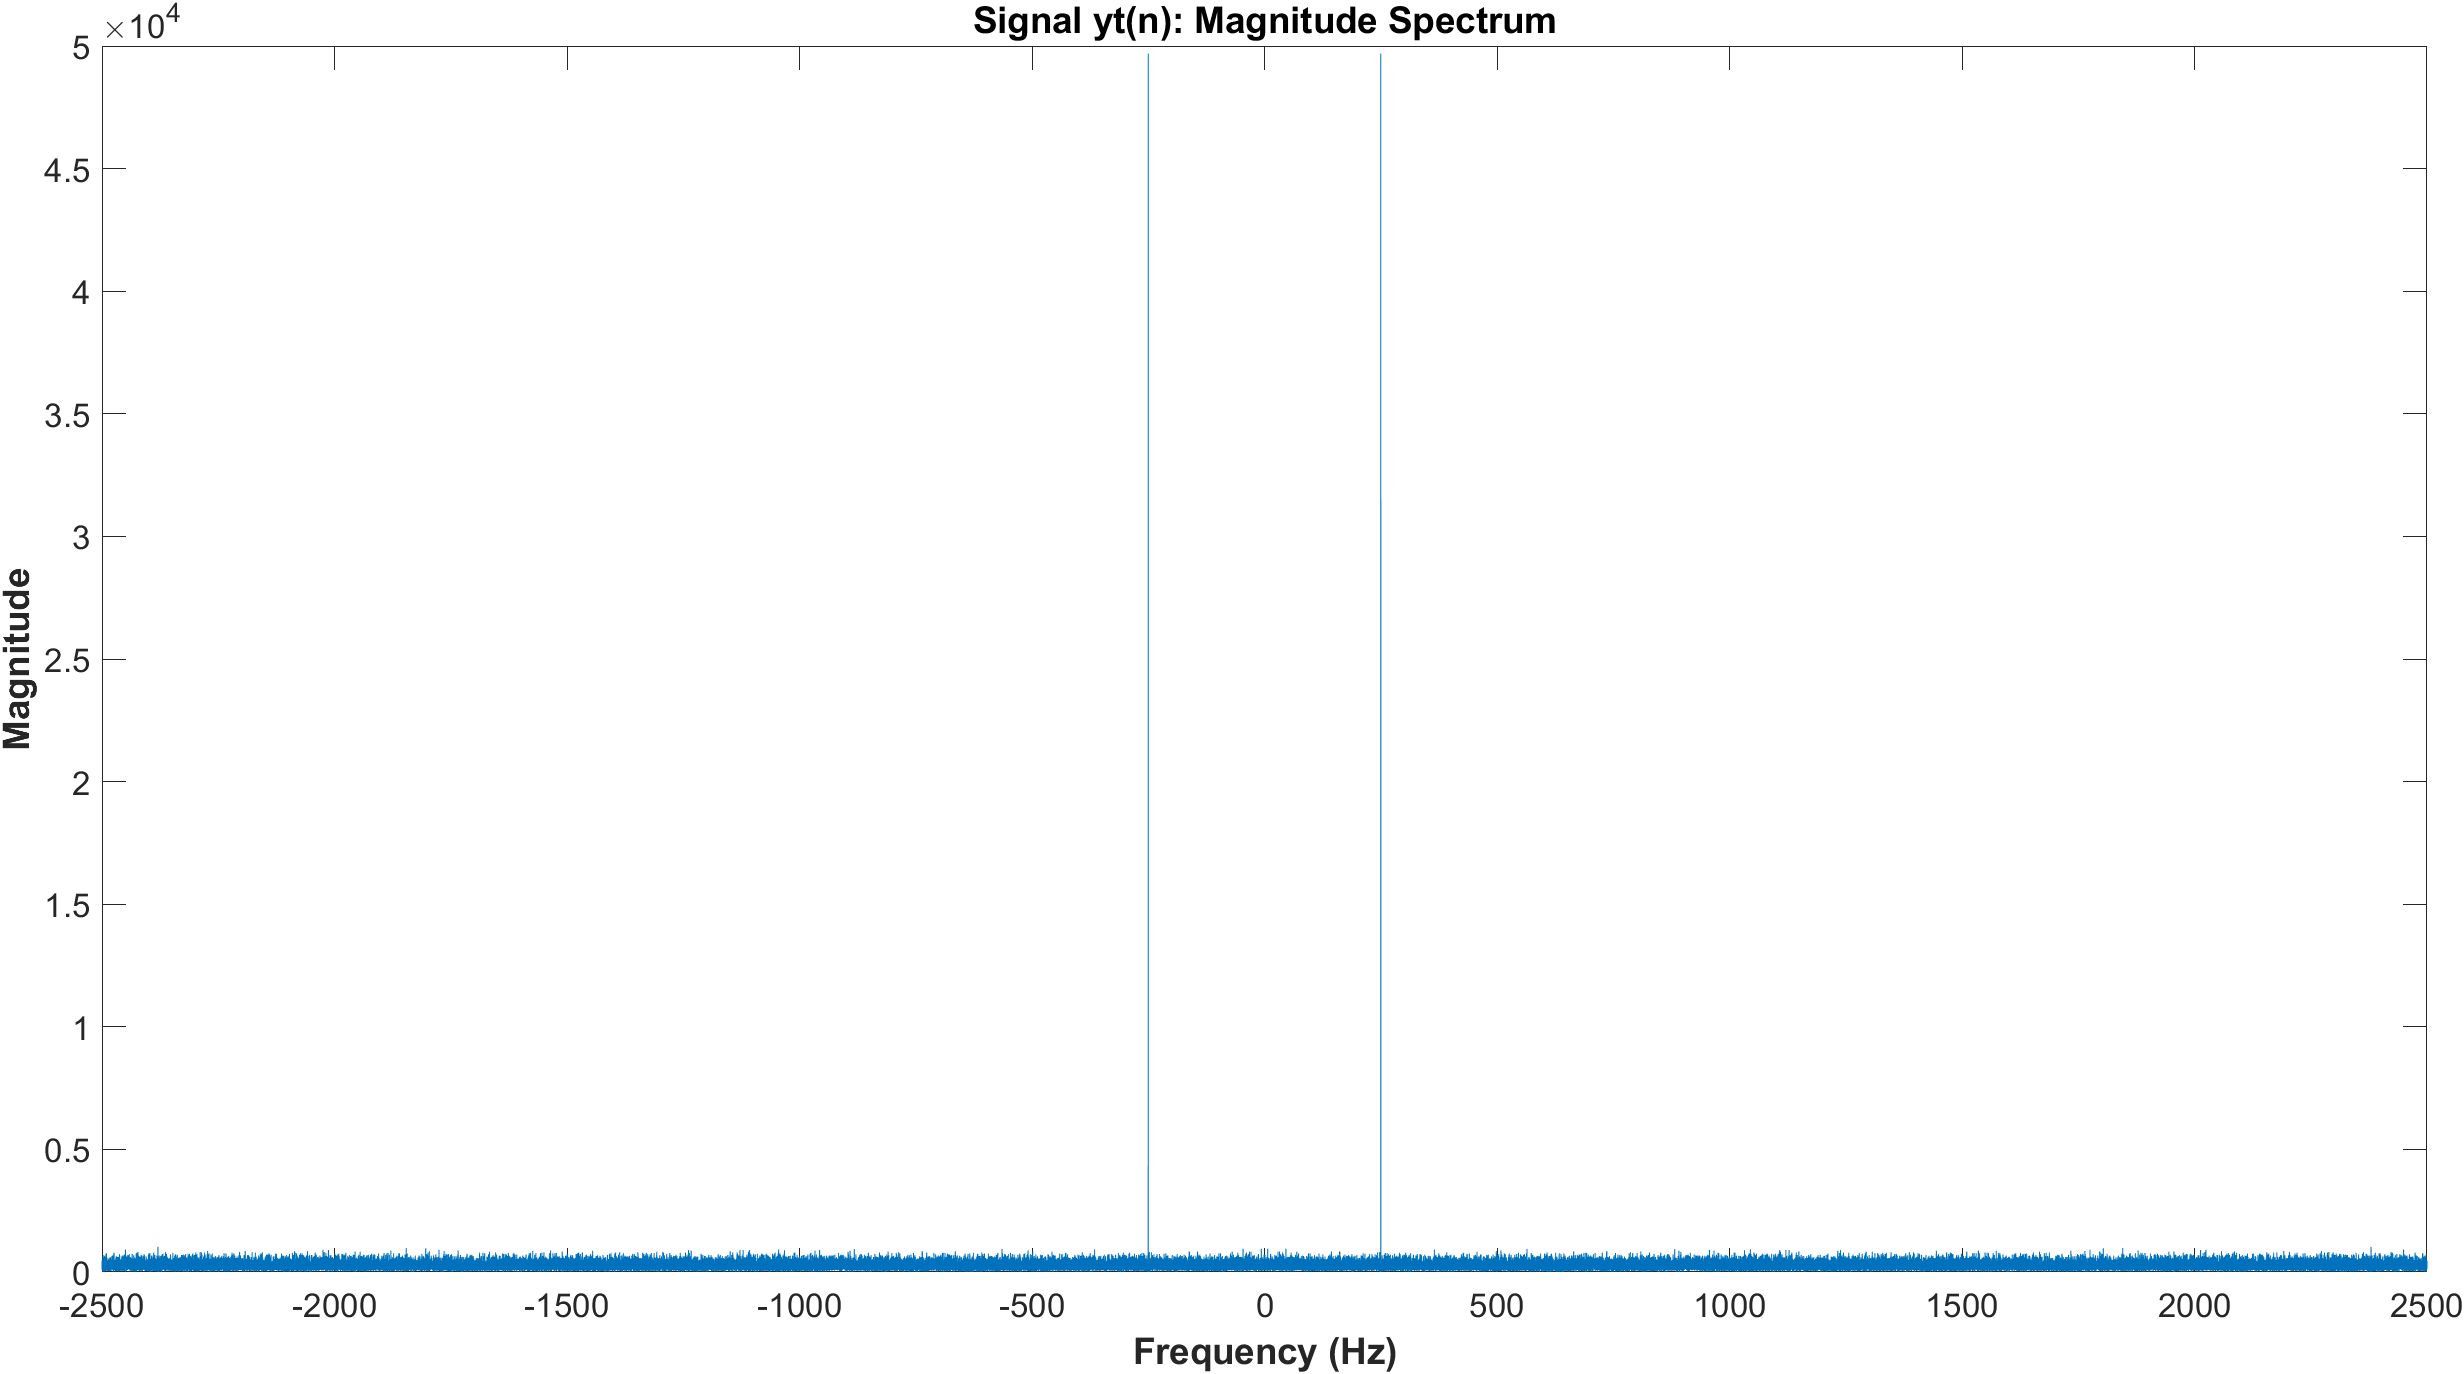
\includegraphics[width=\textwidth]{exp2_fft}
		\caption{\label{fig:exp2_fft}Signal $yt$: Magnitude Spectrum}
	\end{figure}
\end{enumerate}

\section*{Numerical Experiment \#3: Delay Estimation}

% For this section, plot x(t) and y(t) vs time. Explain why your technique works and the straightforward approach of finding the delay by plotting y(t) vs time fails. Provide the plot of cross-correlation between x and y. Can you estimate the delay by the autocorrelation of y(i.e. xcorr(y,y))? Explain.

The signals $x(t)$ and $y(t)$ are plotted in the time domain in Figure~\ref{fig:exp3_time}. From the plot of $y(t)$ in the time domain, it is difficult to determine what the delay is as the signal is almost completely buried in noise. It is difficult to pinpoint the exact location of the peak of the delay due to the noise surrounding it.

An approach to determining the delay would be to plot the cross-correlation between $x$ and $y$, and determining the value of $\tau$ where the autocorrelation function is at its maximum value. The cross-correlation between $x$ and $y$ is plotted in Figure~\ref{fig:exp3_crosscorr}. We can see that the maximum value of the cross-correlation function occurs at $\tau = 0.0424$ seconds. This delay roughly matches the delay found in the time domain plot of $y(t)$ in Figure~\ref{fig:exp3_time}.

The autocorrelation of $y$ (xcorr(y,y)) cannot be used to estimate the delay as the maximum value of the autocorrelation function occurs at $\tau = 0$, which is not equal to the delay in the signal $y$.

\begin{figure}[h]
	\centering
	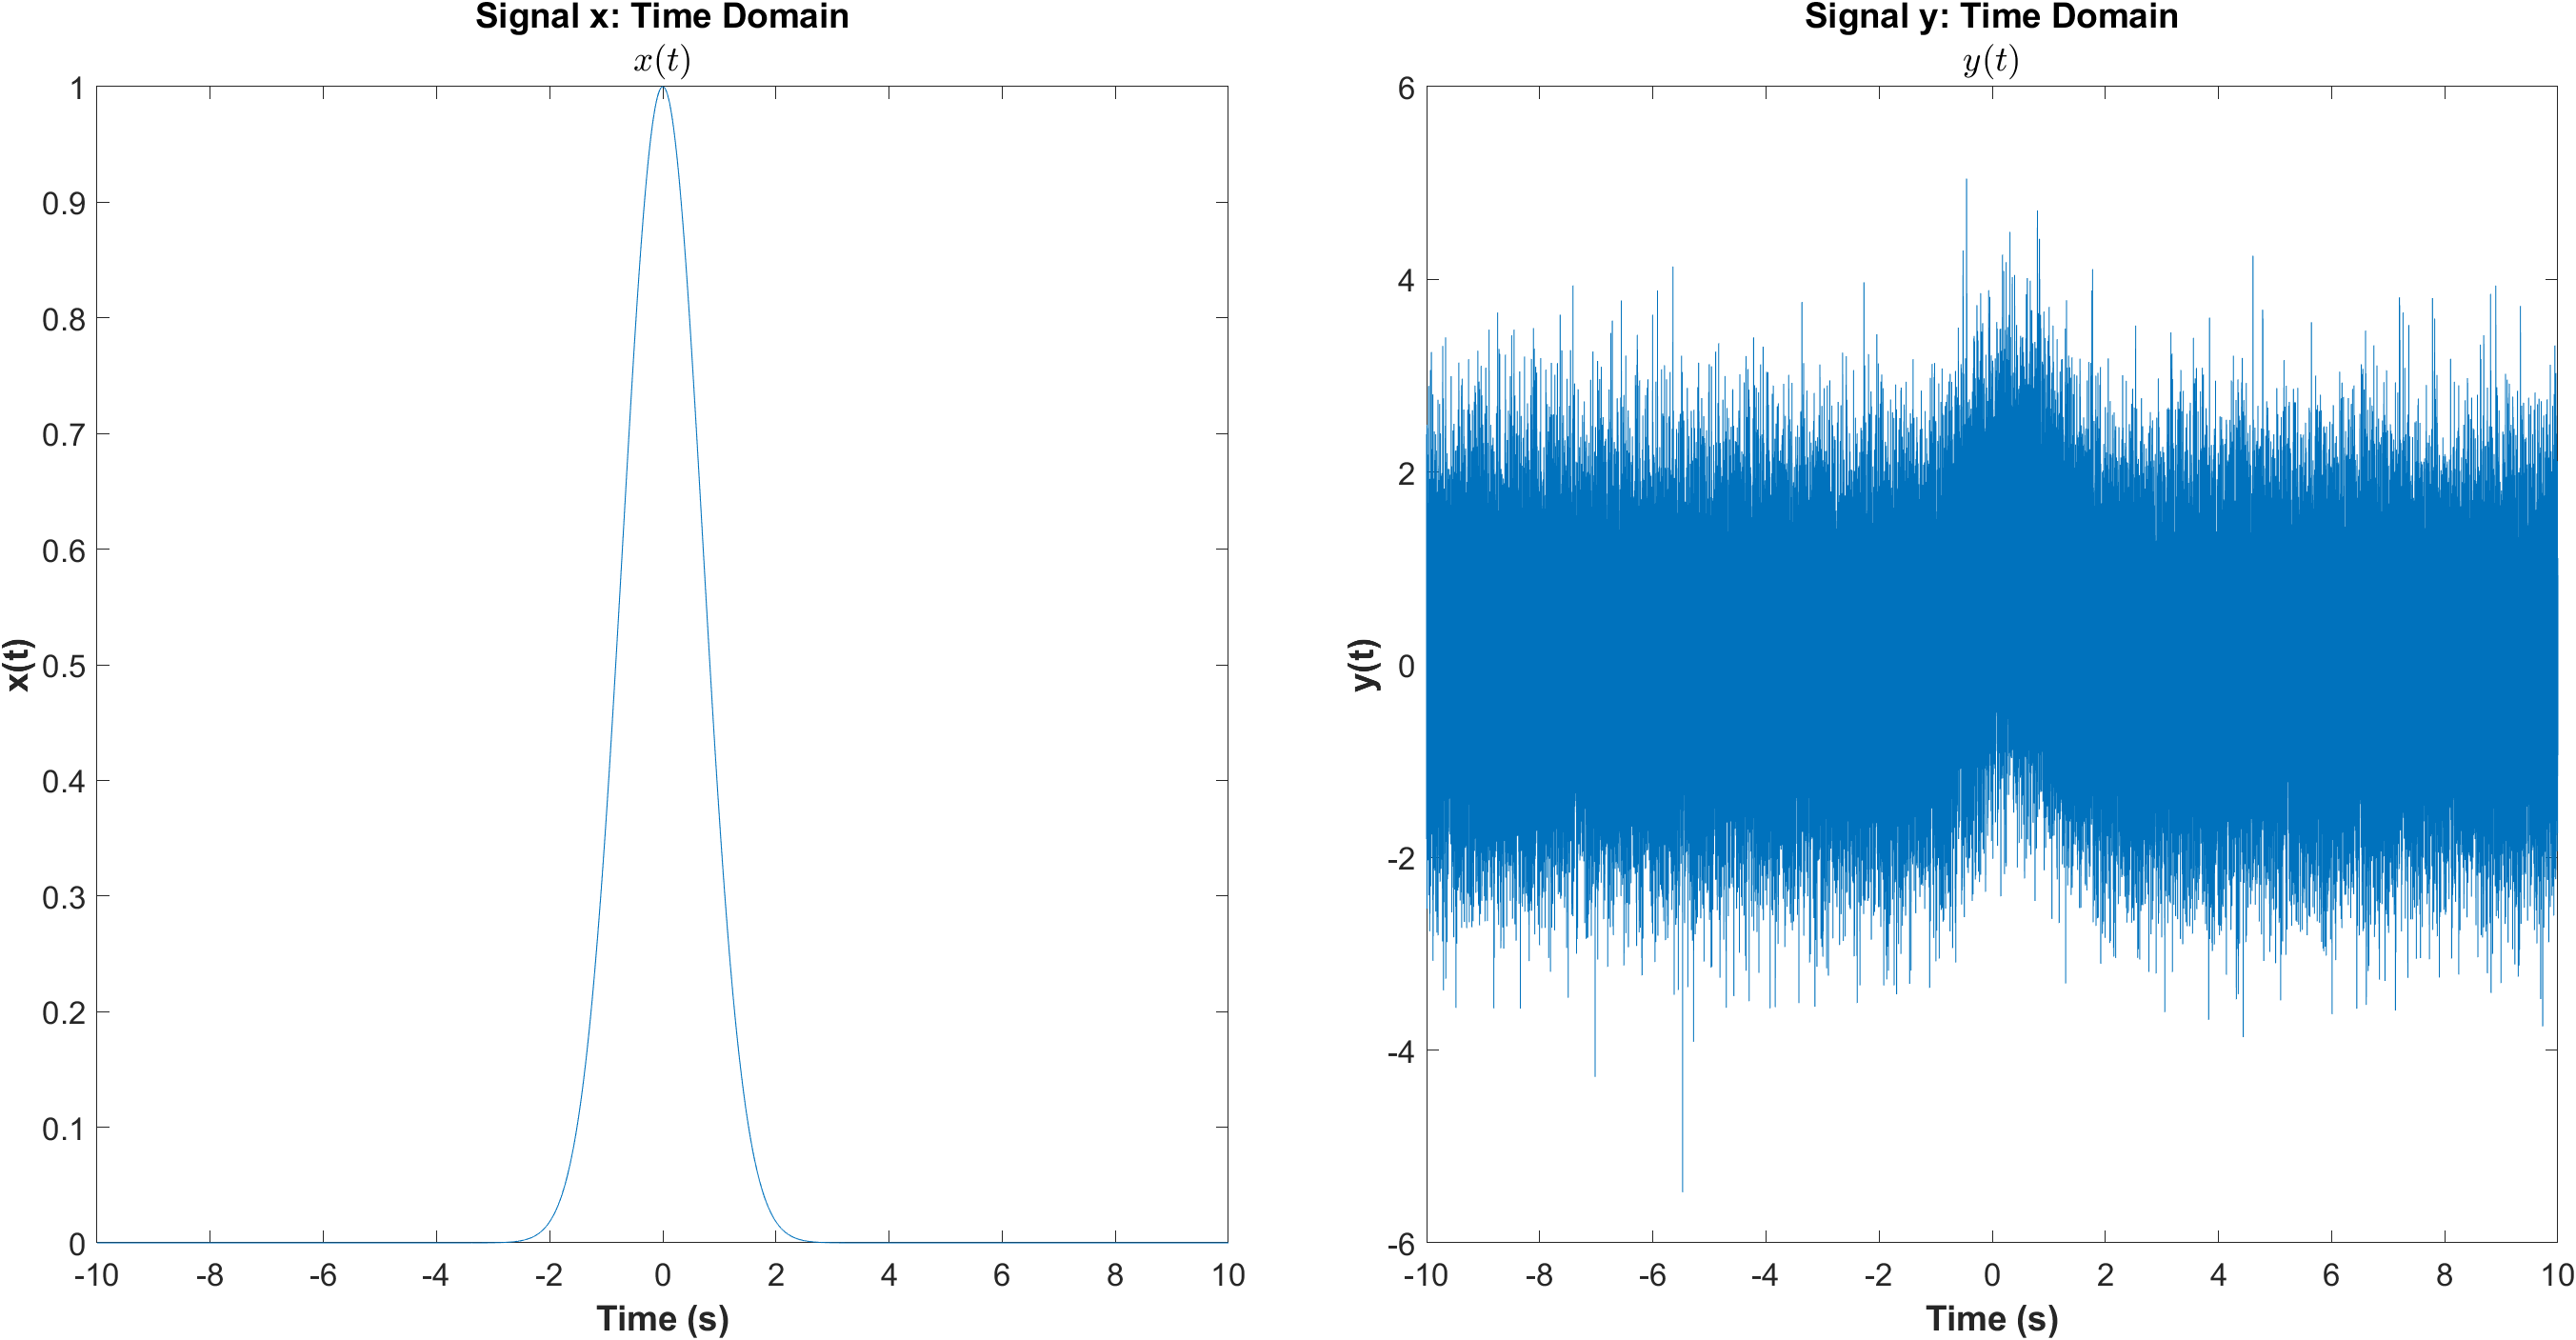
\includegraphics[width=\textwidth]{exp3_time}
	\caption{\label{fig:exp3_time}Signals $x(t)$ and $y(t)$: Time Domain}
\end{figure}

\begin{figure}[h]
	\centering
	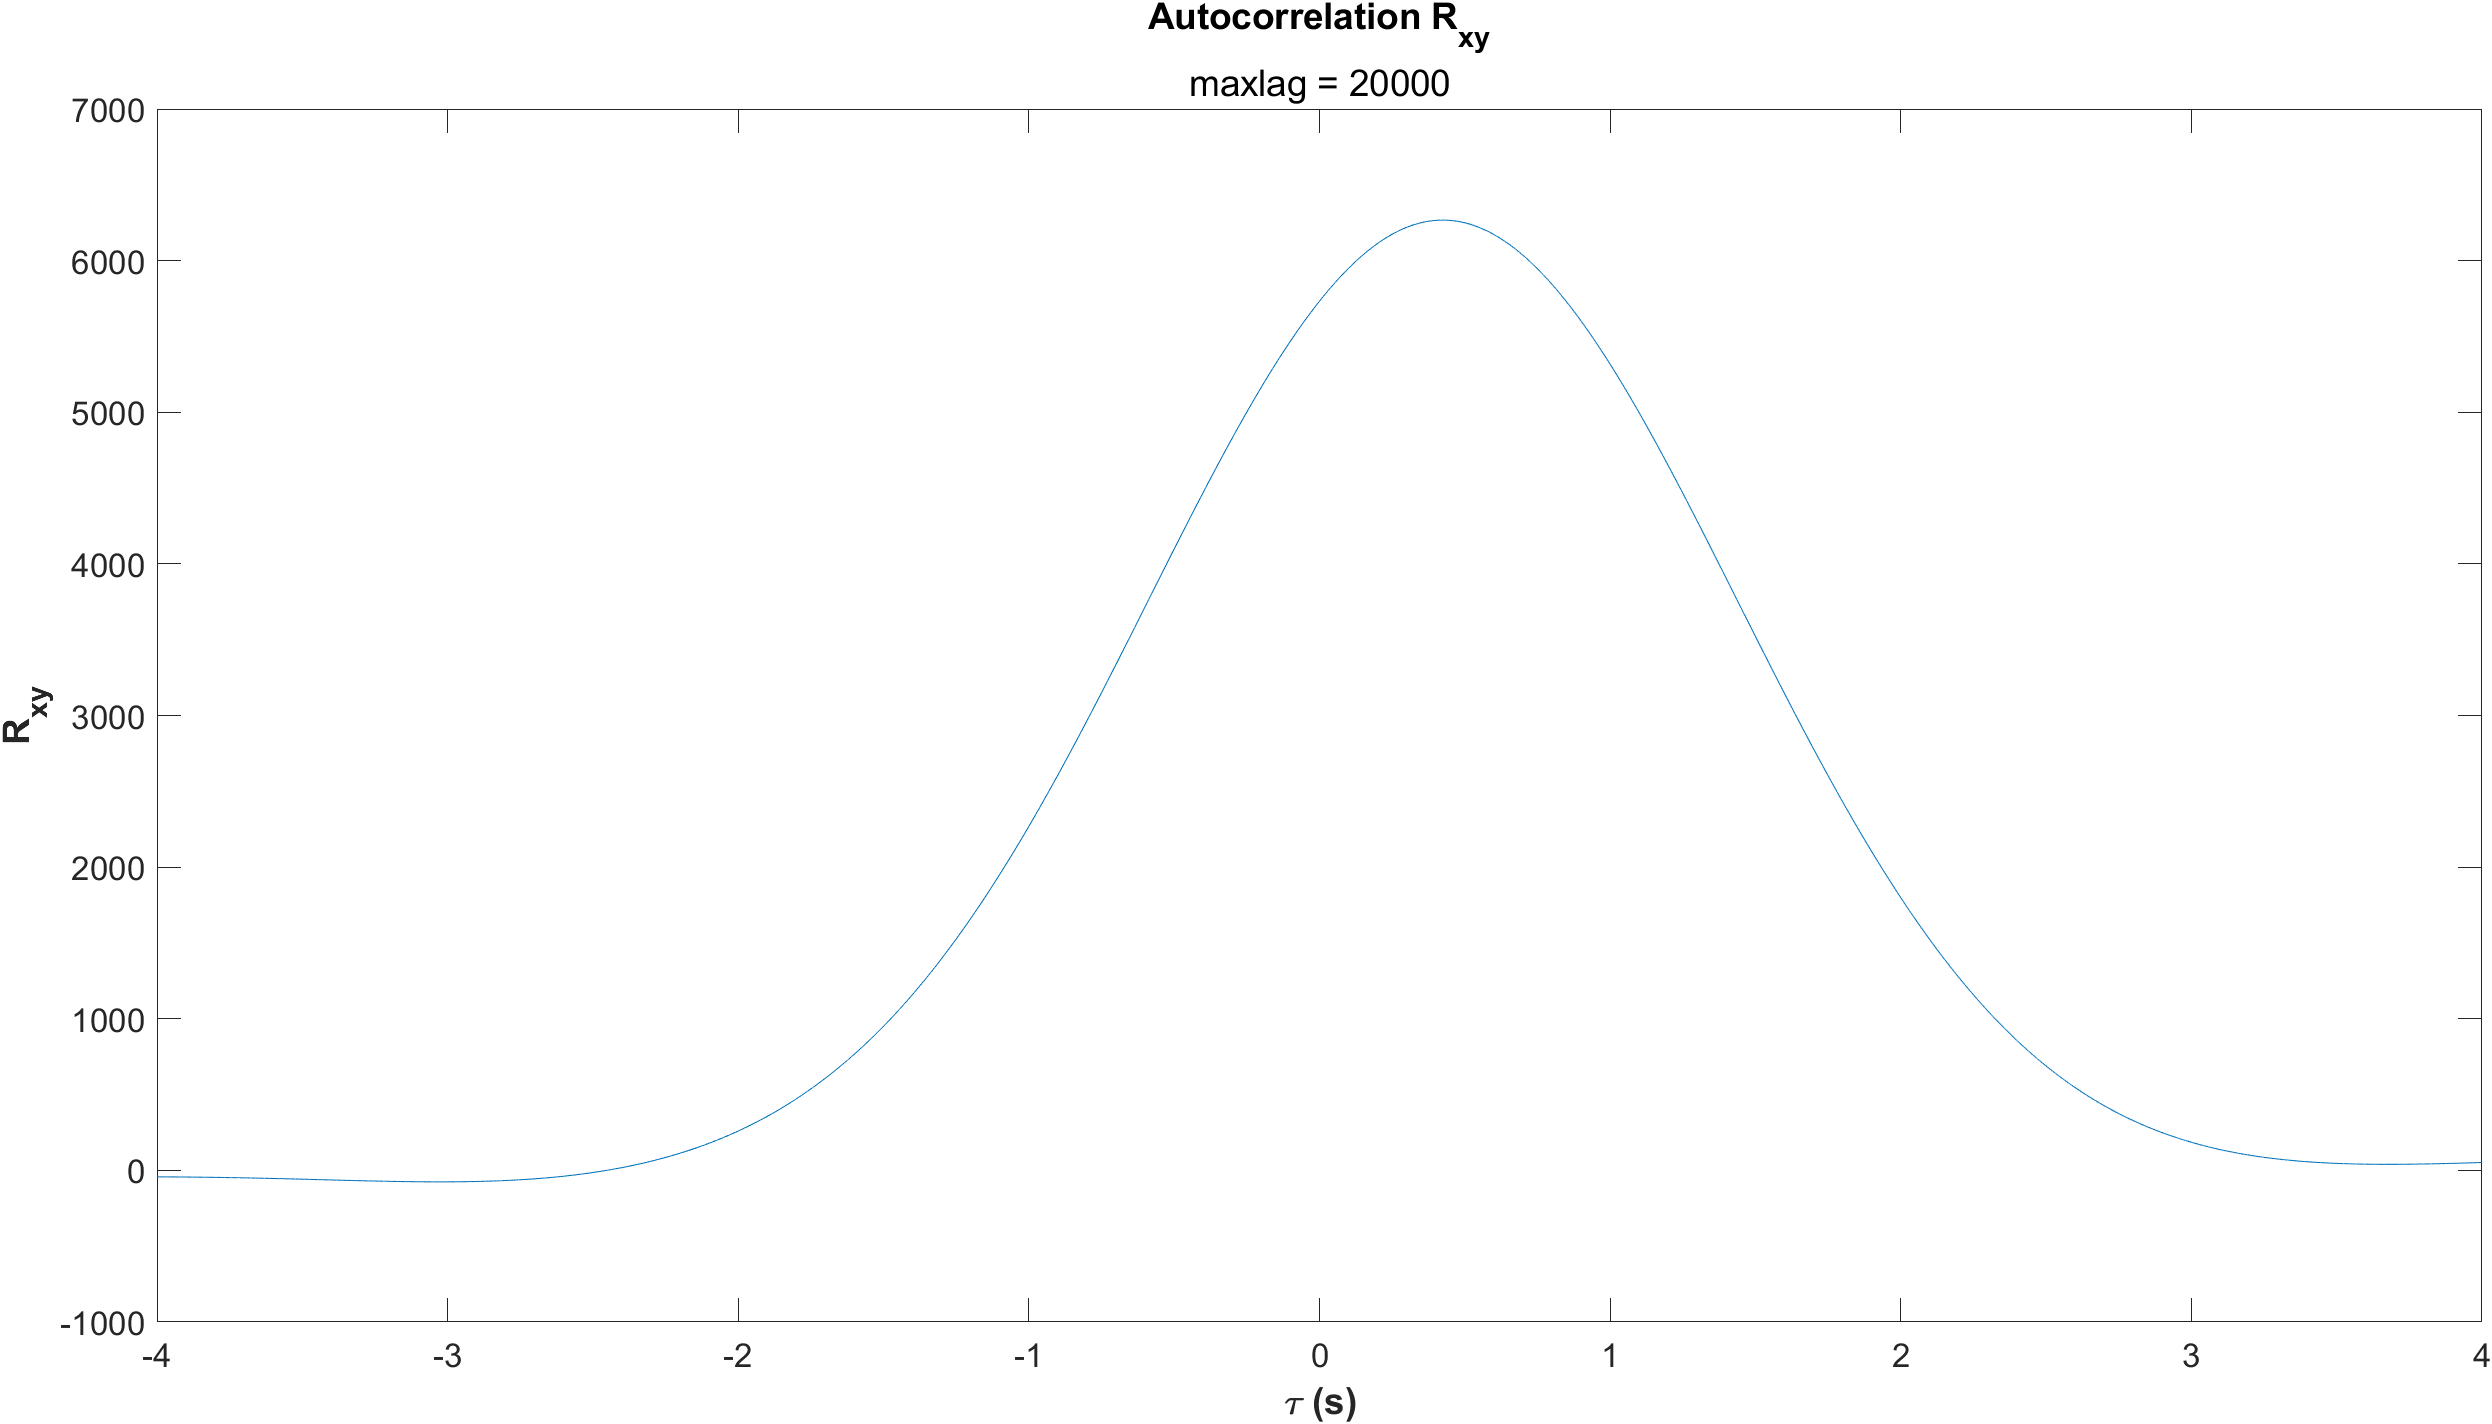
\includegraphics[width=\textwidth]{exp3_crosscorr}
	\caption{\label{fig:exp3_crosscorr}Cross-correlation between $x$ and $y$}
\end{figure}

\end{document}
